% * <rearmstr@gmail.com> 2017-04-26T19:06:47.458Z:
%
% ^.
\documentclass[useAMS,usenatbib]{mnras}

%=====================================================================
% CUSTOM: PACKAGES, MACROS & SETTINGS
%=====================================================================

% packages for figures
\usepackage{graphicx,todonotes}
\usepackage{deluxetable}
% packages for symbols
\usepackage{latexsym,amssymb}
% AMS-LaTeX package for e.g. subequations
\usepackage{amsmath,morefloats}
\usepackage{natbib,graphicx,amsmath,subfigure,color}
\topmargin-1cm
\graphicspath{{figures/}}

\newcommand{\hmsun}{\ensuremath{h^{-1}M_{\odot}}}
\newcommand{\hgpc}{$h^{-1}$Gpc}
\newcommand{\hmpc}{$h^{-1}$Mpc}
\newcommand{\hkpc}{$h^{-1}$kpc}
\newcommand{\beq}{\begin{equation}}
\newcommand{\eeq}{\end{equation}}
\newcommand\notedo[1]{\todo[color=yellow, inline, size=\small]{To do:
    #1}}
\newcommand\notewrite[1]{\todo[color=orange, inline, size=\small]{To write: #1}}
\newcommand\noteask[1]{\todo[color=cyan, inline, size=\small]{To ask: #1}}
\newcommand\notecontrib[1]{\todo[color=green, inline, size=\small]{Contributors: #1}}
\newcommand{\vecM}{\mbox{\boldmath $M$}}
\newcommand{\vecg}{\mbox{\boldmath $g$}}
\newcommand{\vece}{\mbox{\boldmath $e$}}
\newcommand{\veck}{\mbox{\boldmath $k$}}
\newcommand{\vecQ}{\mbox{\boldmath $Q$}}
\newcommand{\vecF}{\mbox{\boldmath $F$}}
\newcommand{\vecD}{\mbox{\boldmath $D$}}
\newcommand{\matR}{\mbox{$\bf R$}}
\newcommand{\matC}{\mbox{$\bf C$}}
\newcommand{\bnab}{\boldsymbol{\nabla}}
\newcommand{\bnabg}{\boldsymbol{\nabla_g}}


%=====================================================================
% FRONT MATTER
%=====================================================================


%=====================================================================
% BEGIN DOCUMENT
%=====================================================================


\title{Measuring weak lensing shear using Bayesian Fourier Domain on 1st Year HSC Data}

\author{Bob Armstrong}

\begin{document}
\date{Draft \today}
\maketitle

\begin{abstract}
We apply the Bayesian Fourier Domain (BFD) method of measuring weak lensing gravitational shear to first year data from the Hyper Suprime-Cam (HSC) survey.  We use deep data from the COSMOS field as a noise free distribution of the underlying galaxy population.  Although the BFD method has been demonstrated to work for low $S/N$ galaxies, we make a conservative selection of objects with magnitude $< 24.6 \Rightarrow S/N \sim 15 $ to avoid potential problems with photometric redshifts.  This results in a number density of 20 galaxies/arcmin$^2$.  We first demonstrate that the method is unbiased in the recovery of the shear on a set of HSC-specific simulations designed to match the observed data.  We then apply the method to the HSC data and look for any systematic errors.  By comparing the measured shear of galaxy clusters we show that the BFD method is completely consistent with the re-Gaussianization method as described in ~\cite{ShearPaper:inprep}.
\end{abstract}


\section{Introduction}

Weak lensing is a powerful tool to constrain both cosmology\citep{2010A&A...516A..63S, 2013MNRAS.432.2433H, DES_CS_cosmology,2017MNRAS.465.1454H} and galactic physics ~\citep{2010ApJ...709...97L, 2012MNRAS.425.2610R, 2017MNRAS.467.3024L}.  It relies on using the change in the measured shapes of galaxies that is imprinted by intervening matter.  The size of the change is sensitive to the total amount of matter.  This is not restricted to visible light and therefore offers a unique probe into the matter content of the universe.  A number of current large surveys (DES, HSC, KIDS) have weak lensing as an integral component in their plan to measure cosmological parameters and the growth of structure.  The challenge in using weak lensing will be ensuring that the various sources of systematic errors are small.  Current surveys are just now gaining enough statistical power that the systematic errors are becoming increasingly relevant.   A lot of work has been carried out in the community to quantify \citep{2006MNRAS.368.1323H,2010MNRAS.405.2044B, 2012MNRAS.423.3163K,  2015MNRAS.450.2963M} and reduce these errors below the expected statistical errors of future surveys.  Among the most pernicious systematic errors are accurate removal of the point spread function (PSF) and biases that come from the shear measurement process itself.  In this paper we focus on the latter.

One common approach to measuring galaxy shear is to use maximum likelihood methods \citep{2013MNRAS.429.2858M, 2016MNRAS.tmp..827J, 2016arXiv160605337F, 2017MNRAS.467.1627F}.  However, in the presence of noise, such methods suffer from noise bias \citep{2012MNRAS.424.2757M,2012MNRAS.425.1951R,2012MNRAS.427.2711K} along with other more subtle biases such as model \citep{2010MNRAS.404..458V} and selection bias.   To correct these biases, it is usually necessary to create carefully tuned simulations to derive calibration factors.  In \cite{Bernstein2015,Bernstein2016}, we proposed an alternative method, Bayesian Fourier Domain (BFD), to overcome these problems.  We showed initial results based on semi-realistic simulations that were able to reduce the multiplicative bias on the shear to the level of $2\times 10^{-3}$, close the requirements for future large scale surveys such as LSST and Euclid.  While these results are encouraging, the method has not yet been demonstrated on real data.  This paper applies the BFD approach to the first year data from the Hyper Suprime-Cam (HSC) survey.

The Hyper Suprime-Cam (HSC) \citep{SurveyOverview} survey is a galaxy survey using the Subaru telescope to eventually observe $\sim$1400 deg$^2$.  Due to the large telescope and excellent seeing it will reach a 5$\sigma$ point source depth of 26.5.  The recently released first year HSC data \citep{DataPaper:inprep} comprises $\sim$170 deg$^2$ of full depth data, providing an excellent dataset for weak lensing.  In \cite{ShearPaper:inprep} the re-Gaussianization \citep{2003MNRAS.343..459H} shear estimation method was applied to the HSC data and the corresponding shear catalog was presented.  In the re-Gaussianization method, galaxy moments are PSF-corrected assuming a Gaussian PSF.  Corrections are the applied for the dilution of the observed shape by the PSF and deviations of the PSF from Gaussianity.  It relies on calibration factors, derived from simulations, on the order of $\sim10\%$ to correct for the inherent biases of the method.  The main advantage of BFD is that it does not rely on external simulations and has very different assumptions.  Agreement between the two methods serves as an important cross-check of the re-Gaussianization method.

In Section \ref{Sec:Overview}, we give a simplified overview of the BFD method and how it was specifically applied to HSC.  Section \ref{Sec:Prior} describes the creation of priors on galaxy moments from deep HSC data.  We demonstrate the application of the method on a suite of HSC based simulations in Section \ref{Sec:Sims}. Section \ref{Sec:Data} shows a number of validation tests that can be measured directly from the data.  We compare results from the BFD with re-Gaussianization in Section \ref{Sec:Comparison}.  Finally, we summarize how to use the catalog, known issues and planned improvements to the method for future releases.

\section{Overview of Method}
\label{Sec:Overview}

In the Bayesian Fourier Domain (BFD) method \citep{Bernstein2015,Bernstein2016}, we do not attempt to measure the shear of individual galaxies, but rather the likelihood of the pixel data given a particular shear \vecg.  For each galaxy we compress the pixel data into a set of moments, $\vecM$, in Fourier space:
\begin{equation}
\label{moments}
\vecM \equiv \left( \begin{array}{c}
M_f \\
M_r \\
M_+ \\
M_\times
\end{array}
\right) = \int d^2k\, \frac{\tilde I^o(\veck)}{\tilde T(\veck)}
W(|\veck^2|) \vecF; \quad \vecF \equiv
\left( \begin{array}{c}
1 \\
k_x^2 + k_y^2 \\
k_x^2 - k_y^2 \\
2 k_x k_y
\end{array}
\right).
\end{equation}
where  $\tilde I^o$ is the Fourier transform of the image, $\tilde T(\veck)$ is the Fourier transform of the PSF and  $W(|\veck^2|)$ is a window function to bound the noise.  We assume that the covariance matrix of these moments is a multivariate Gaussian.  (When is this not true?) We can use Bayes' theorem to calculate the posterior of the shear, \vecg,
given the observed moments:
\begin{equation}
P(\vecg | \vecM) = \frac{P(\vecM | \vecg) P(\vecg)}{P(\vecM)}.
\end{equation}
If we assume that the applied shear is weak and do a second order Taylor expansion around $\vecg=0$:
\begin{align}
P(\vecM | \vecg) & = P + \vecQ\cdot \vecg + \frac{1}{2} \vecg \cdot
\matR \cdot \vecg, \\
P & \equiv P(\vecM | \vecg=0)  \\ \label{q1eqn}
\vecQ & \equiv \left.\bnabg P(\vecM | \vecg)\right|_{\vecg=0} \\
\matR & \equiv \left. \bnabg \bnabg P(\vecM | \vecg)\right|_{\vecg=0}.
\end{align}
For simplicity, the above expression ignores the probability that an object is detected and selected.  The full expression can be found in \cite{Bernstein2016}.  For a set of galaxies with the same applied shear, we can compute $P_i, \vecQ_i, \matR_i$ for each galaxy.
The posterior becomes:
\begin{align}
-\ln P(\vecg | \vecD) & = (\rm const) - \ln P(\vecg) - \sum_i \ln P(\vecD_i | \vecg) \\
\label{pqr1}
 & =  (\rm const) - \ln P(\vecg) - \vecg \cdot \vecQ_{\rm tot}
+ \frac{1}{2} \vecg \cdot \matR_{\rm tot}
   \cdot \vecg, \\
\label{eqn:qtot}
\vecQ_{\rm tot} & \equiv \sum_i   \frac{\vecQ_i}{P_i} \\
\label{eqn:rtot}
\matR_{\rm tot} & \equiv \sum_i \left(
   \frac{\vecQ_i\vecQ_i^T}{P_i^2} - \frac{\matR_i}{P_i}\right)
\end{align}
Assuming the data is more informative than the prior on \vecg, the posterior is Gaussian with covariance matrix
$\matC_g = \matR_{\rm tot}^{-1}$ and mean value $\bar\vecg = \matR_{\rm tot}^{-1} \vecQ_{\rm tot}$.

In measuring $P_i, \vecQ_i, \matR_i$ we need to know how the true, noise-free distribution of moments responds to shear
\begin{equation}
P(\vecM|\vecg) = \int  d\vecM_{\rm true} P(\vecM|\vecM_{\rm true})P(\vecM_{\rm true}|\vecg)
\label{trueM}
\end{equation}
and its corresponding derivatives.  These can be computed analytically using deep high-$S/N$ observations.

In order to evaluate the integral in Equation \ref{trueM}, we approximate the full galaxy moment distribution as a sum of $\delta$ functions from individual galaxies in the deep field.  Because of parity and rotation symmetry of the un-lensed sky, we are free to increase the number of galaxies by adding rotated and parity-transformed copies of galaxies.  We store the moments of these galaxies in a $k$-d tree for fast searching.  With these in hand, we can use kernel density estimation with the moment likelihood as the smoothing kernel.  Operationally, we sample from the set of prior galaxies with moments within some $\chi^2$ of the measured $\vecM$.  One complication with this is that galaxies with high $S/N$ will have a small kernel and the prior galaxies are more sparse at bright magnitudes.  To overcome this, we add additional measurement noise to the galaxy moments, thus increasing the number of prior objects that it will overlap with.  For a more complete discussion of this procedure see \cite{Bernstein2016}.


\section{Application to HSC}

As a starting point, we use the fully reduced HSC coadded data. \citep{CatalogPaper:inprep} describes the process of detrending on single visits, PSF modeling, astrometric registration, coaddition and object detection and deblending in detail.  In this analysis, we utilize images from the $i$-band data, as that filter was specifically chosen to have the best seeing.  

Here is a brief overview of the process for running BFD on HSC data:
\begin{itemize}
\item Measure the moments in Fourier space for all objects using Equation \ref{moments}.  
\item Group objects together with similar moment covariance matrices.  Compute the average moment covariance matrix for each group as input to deriving the prior.
\item Given a moment covariance matrix, measure moments and their derivatives with respect to shear on a set of deep observations.  Create a set of prior objects for each covariance matrix. 
\item Using the deep observations, measure the selection probability and its derivatives given the flux selection cuts.
\item For galaxies from each group, use the appropriate moment priors and measure $PQR$.
\item Create a selection catalog based on a pixelization of the survey geometry and the selection probabilities.
\end{itemize}
Each item will be explained in further detail hereafter. 

\subsection{Moment Measurements}
Moments are measured given an initial centroid on the fully deblended image.  Pixels not associated with the object in the image have been replaced with noise.  After the initial moment measurement, we shift position of the center such that the centroid moments are nulled.  If the shifted centroid is farther than 4 pixels away from the initial centroid this object is flagged.  This happens most often when an object was detected in a band other than the $i$-band.

We select the weight function to be the same for all objects.  It is defined as:
\begin{equation}
\label{ksigma}
W\left(|k^2|\right)  \equiv \left\{ 
\begin{array}{cc}
\left( 1 - \frac{k^2\sigma^2}{2N}\right)^N & k <\frac{\sqrt{2N}}{\sigma} \\
0                                          & k \ge \frac{\sqrt{2N}}{\sigma} 
\end{array}
\right.
\end{equation}
This weight function has two free parameters: the index $N$ and $\sigma$.  We choose $N=4$ and optimize $\sigma$ to maximize the moment $S/N$ for a typical galaxy in HSC.  The resultant value is $\sigma=2$ pixels.

All BFD measurements are currently done in pixel coordinates.  The final $PQR$ values are then rotated to be in sky coordinates.  Given that the astrometric registration is done in regions of sky 0.25\arcmin$\times$0.25\arcmin, there can be some distortion across an individual field making the conversion to sky coordinates more complicated than a simple rotation.  However, the maximum change in shear values from such distortions is small ($\sim 10^{-4}$) and therefore currently ignored.  Future versions of the code will avoid the need for this rotation by doing measurements directly in sky coordinates.

\subsection{Measuring Noise}
\label{Sec:Noise}
When calculating the $PQR$ values, we need the pixel variance for each object to compute the moment covariance matrix.  The coadded images themselves carry a variance map, however this variance does not account for the covariance between pixels from the interpolation.  There is also an attempt to rescale the variance map of each coadded image to account for the missing variance lost due to covariance.  This complicates the use of the variance map.  Instead, we choose to measure the variance locally for each object by growing the detection footprint around each object and calculating the variance of the pixels not found in the detection mask.  The footprint is grown by factors of 2, up to a maximum of 8, until there are more than 100 pixels not flagged in the detection mask.  When an insufficient number of pixels is found these objects are flagged.  This happens most frequently with junk detections around bright stars.

We can compare the variance estimates measured this way to the values from the coadded variance map.  We take the median value of the variance map from the objects bounding box (note, this was how the noise was measured for the re-Gaussianization method) and then scale by the appropriate factor for each patch that we found in the HSC processing logs as this information was not stored in the files.  Figure\ref{fig:noise_compare} shows the ratio of the variances from the coadd maps to our method.  We see that our method measures a larger variance by $\sim10\%$.  This could potentially come from pixels around the outskirts of galaxies that have flux but were below the detection threshold and thus incorrectly included in our method.  To test the potential effect of mis-estimating the pixel noise, we tested our shear algorithms on simulations (see Section\ref{Sec:Sims} where we artificially increased the pixel noise from the true value by $10\%$ and saw no detectable bias in the measured shear.  We did the same thing for the actual data and measured the shear signal around galaxy clusters (see Section\ref{Sec:Comparison}).  We also saw no statistically significant change in the lensing signal.  Thus, if we are indeed wrong in the variance calculation it should not significantly impact the result.


\begin{figure}
    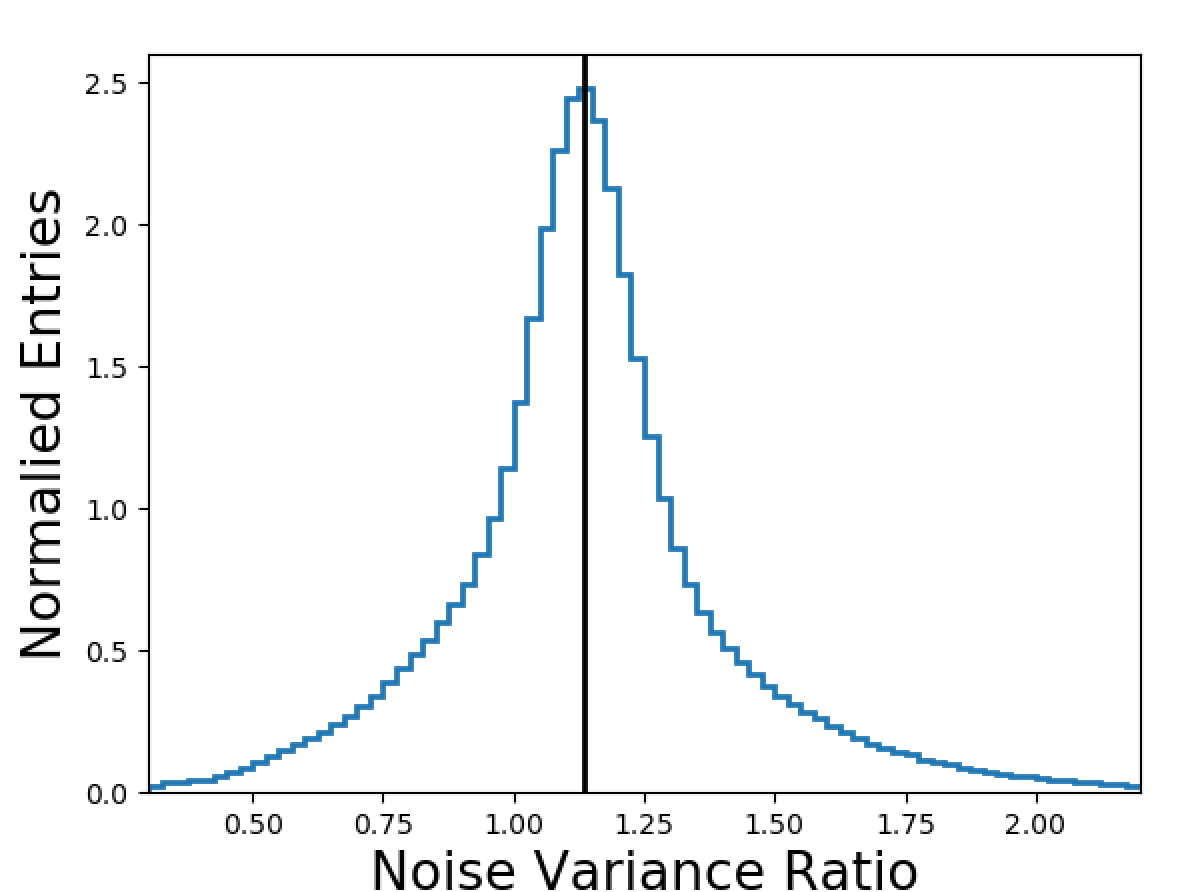
\includegraphics[width=0.5\textwidth]{noise_compare.png}
    \caption{
       The ratio of the pixel variance as measured by taking the average of noise pixels around objects compared to the value obtained from the coadd variance map.  We see that our method measures the variance to be $\sim10\%$ larger. 
    }
    \label{fig:noise_compare}
\end{figure}



The coaddition process introduces pixel correlations when resampling to a common grid.  If not properly accounted for, this can lead to biases in the shear at the level of $2-3\%$ (see Section \ref{Sec:Sims}).  Due to the limited information from the pixels used for the variance calculation around each object, we calculate the correlations on average, over the whole survey.  In the presence of correlations, the moment covariance matrix, $\matC_M$, becomes:

\begin{equation}
\left(\matC_M\right)_{ij} = 
\int d^2k\, P_n(\veck) \left| \frac{W(|\veck^2|)}{\tilde T(\veck)}
\right|^2 F_i(\veck) F^\star_j(\veck),
\label{eqn:cov}
\end{equation}

where $P_n(\veck)$ is the noise power spectrum.  To find the noise correlation power spectrum we choose blank fields from the full survey of size 21x21 pixels.  These fields are chosen by randomly placing 200 points in each patch. If the field has $> 95\%$ of its pixels unmasked (i.e. not flagged as problematic or part of a detected object) we compute the pixel covariance of the unmasked pixels, otherwise the field is ignored.  We then average the correlation over all blank fields and compute the correlation power spectrum.  The observed spectrum matches our expectation of a third order Lanczos interpolation kernel.  

In Figure \ref{fig:noise_ps}, we plot the average noise correlation power spectrum.  The error bars represent the variance from the different tracts.  While there are small variations, it is quite constant across the survey.  The plot also shows the power spectrum for the tract with the maximum deviation from the average.  The largest discrepancy is seen in the low $\veck$ bin indicating a potential problem with background subtraction.  The resultant noise correlation power spectrum can be scaled by the pixel variance for each object and inserted into Equation \ref{eqn:cov}. 


\begin{figure}
    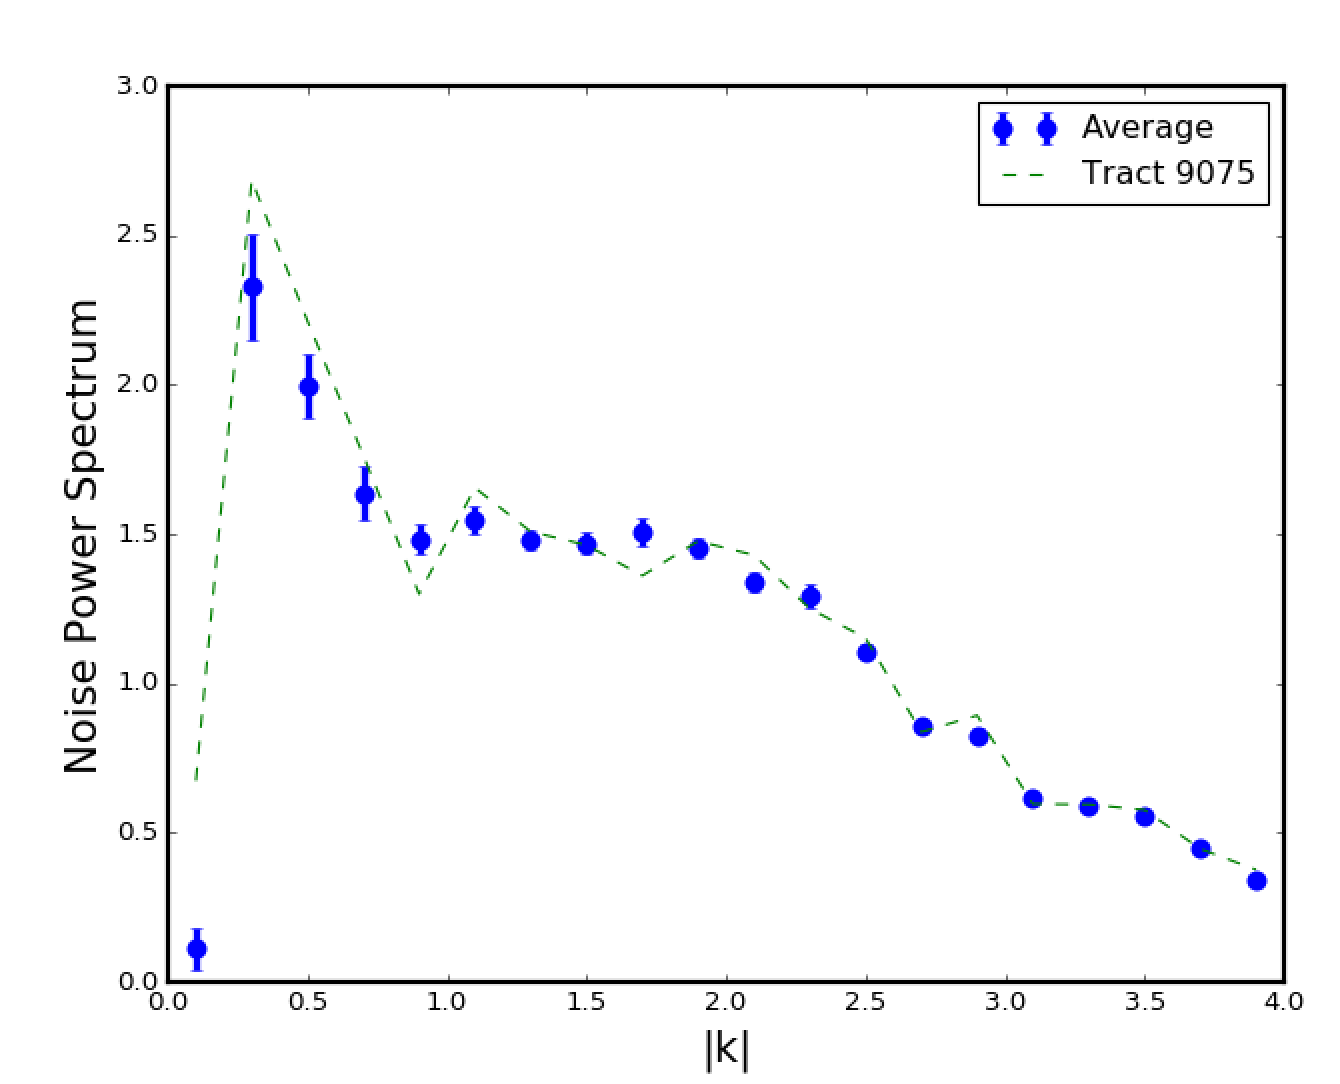
\includegraphics[width=0.5\textwidth]{noise_ps.png}
    \caption{
       The noise power spectrum as a function of $|\veck|$, averaged over blank fields in all the tracts.  The error bars represent the spread among the different tracts.  The tract with the largest deviation from the average, Tract 9075, is also shown.
    }
    \label{fig:noise_ps}
\end{figure}

\subsection{Selection Cuts}

For BFD, we model the shear selection function using only a minimum and maximum flux cut.  As shown in \cite{Bernstein2016}, BFD can accurately measure shear from poorly measured galaxies down to $S/N=5$. However, for this analysis we restrict ourselves to a galaxy sample with magnitude $\le 24.6$, which has $S/N\approx20$.  The primary reason for this is because of the unknown quality of photo-zs fainter than this magnitude.  In the faint galaxy regime, there few spectroscopic redshifts, requiring the photo-z algorithms to rely on grism and high quality photo-zs for training and validation.  To avoid any potential problems with photo-z quality we choose a rather conservative cut.  The conservative cut was also motivated by a similar cut made in \cite{ShearPaper:inprep} for the re-Gaussianization method.  In that paper, a CModel, $i$-band magnitude cut of $\le 24.5$ was used as the minimum magnitude cut.  Because the CModel algorithm allows additional degrees of freedom, galaxy magnitudes will be brighter than those measured for BFD.  Near the 24.5 cut, BFD magnitudes are $\sim0.1$ magnitudes fainter, we therefore use a minimum flux cut of 24.6.  In this manner, the same photo-z validation can be used for both catalogs, reducing the effort needed for scientific analyses.

To include brighter, higher $S/N$ objects we would have to add additional complexity by including additional priors with extra added measurement noise.  To reduce the number of additional priors needed, we choose a maximum $S/N$ of 80, which, given a moment covariance matrix, can be used to find the maximum flux.

%Figure \ref{fig:bfd_cmodel} shows the average difference between these fluxes.  At magnitude 24.5, we see a typcial offset of 0.1 mags.  
%We therefore choose our minimum magnitude cut at 24.6.

%\begin{figure}
%    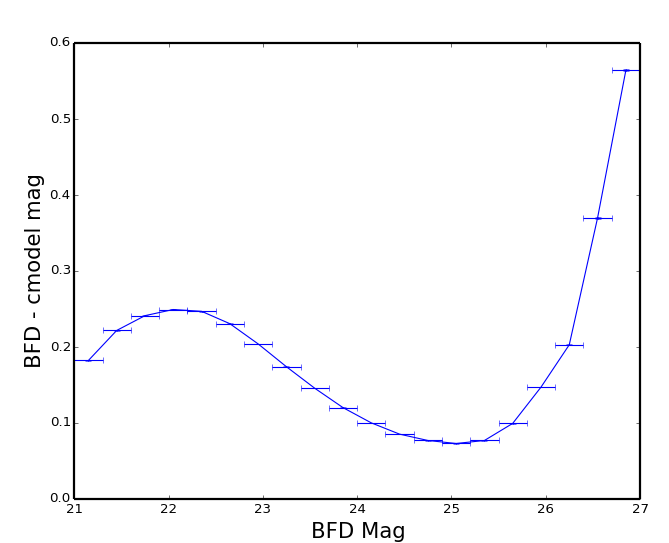
\includegraphics[width=0.5\textwidth]{bfd_cmodel_data.png}
%    \caption{
%      Average difference of BFD magnitudes with cmodel.  
%    }
%    \label{fig:bfd_cmodel}
%\end{figure}


\subsection{Grouping objects with similar Covariances}
The current BFD implementation assumes that the moment covariance matrix is already known before building the prior.  This is needed in two places in the code.  First, we scale the moments of prior objects in the $k$-d tree by the Cholesky decomposition of the covariance matrix so that the $\chi^2$ between galaxies and prior galaxies can be computed easily. It also allows us to significantly reduce the number of prior galaxies we need to keep in memory by rejecting those that will not significantly contribute to the integral in \ref{trueM}.

Because the coadded HSC data has pixel noise and PSF that varies from position to position, we first divide the data into groups where the covariance does not vary by more than $\sim5\%$.    We found that the variance in the flux scales well with the variances of the second moments.  Meaning, that we can use the flux variance to group objects.  Results from simulations show this accuracy is sufficient to remove bias (see Section \ref{Sec:Sims}) below the level required for first year HSC science. In Figure ~\ref{fig:flux_var}, we show the flux variance for the Wide, Full-Depth-Full-Color (FDFC) Wide and Ultra-Deep data.  The FDFC region is defined in \cite{ShearPaper:inprep}.  This indicates regions where we have obtained sufficient colors and depth in all five filters.   We see that the Ultra-Deep data is less noisy as expected, but that the FDFC region still has a large dynamic range similar to the full Wide data.  This may be partly due the definition of the FDFC region, which is defined in terms of the number of exposures taken at a particular location, instead of explicitly choosing depth.  We divide the data into 23 bins of width 0.05 from 0.05 to 1.20.  This selection rejects 13$\%$ of the total galaxies, but only 0.7$\%$ of the FDFC region. Figure \ref{fig:radec_noise_bin} shows the noise bin (from 1-23) as a function of position for the six different observed regions.

\begin{figure}
    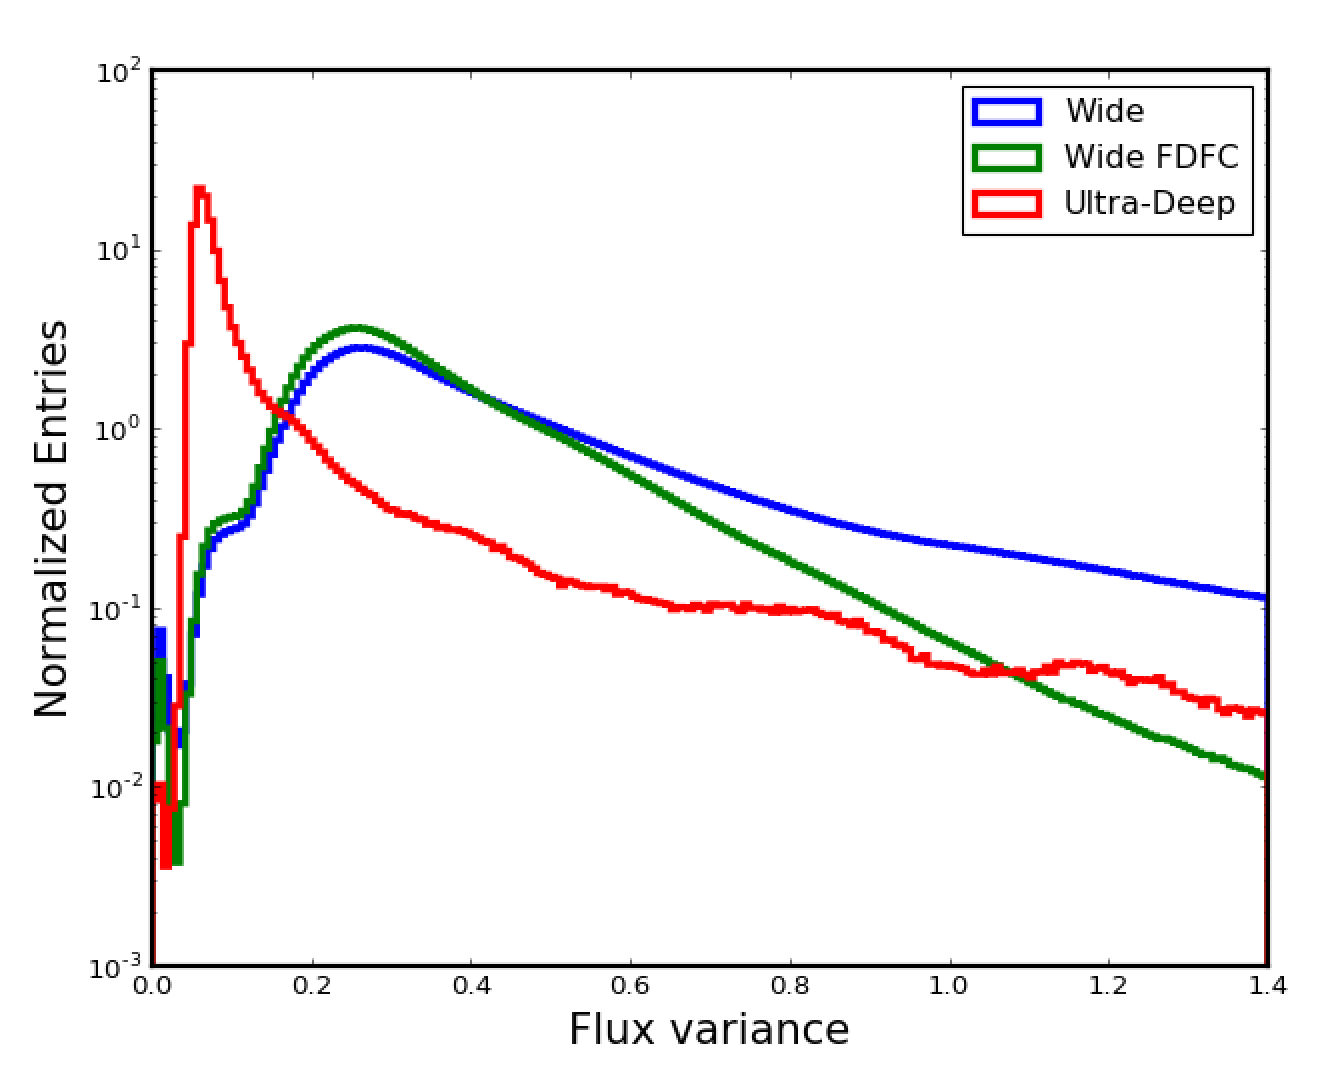
\includegraphics[width=0.5\textwidth]{flux_var.png}
    \caption{
       The distribution of BFD flux variances for different samples: Wide, Wide FDFC (Full-Depth-Full-Color), and Ultra-Deep.  We select galaxies with variance between 0.05 and 1.2 for our analysis.
    }
    \label{fig:flux_var}
\end{figure}


\begin{figure*}
    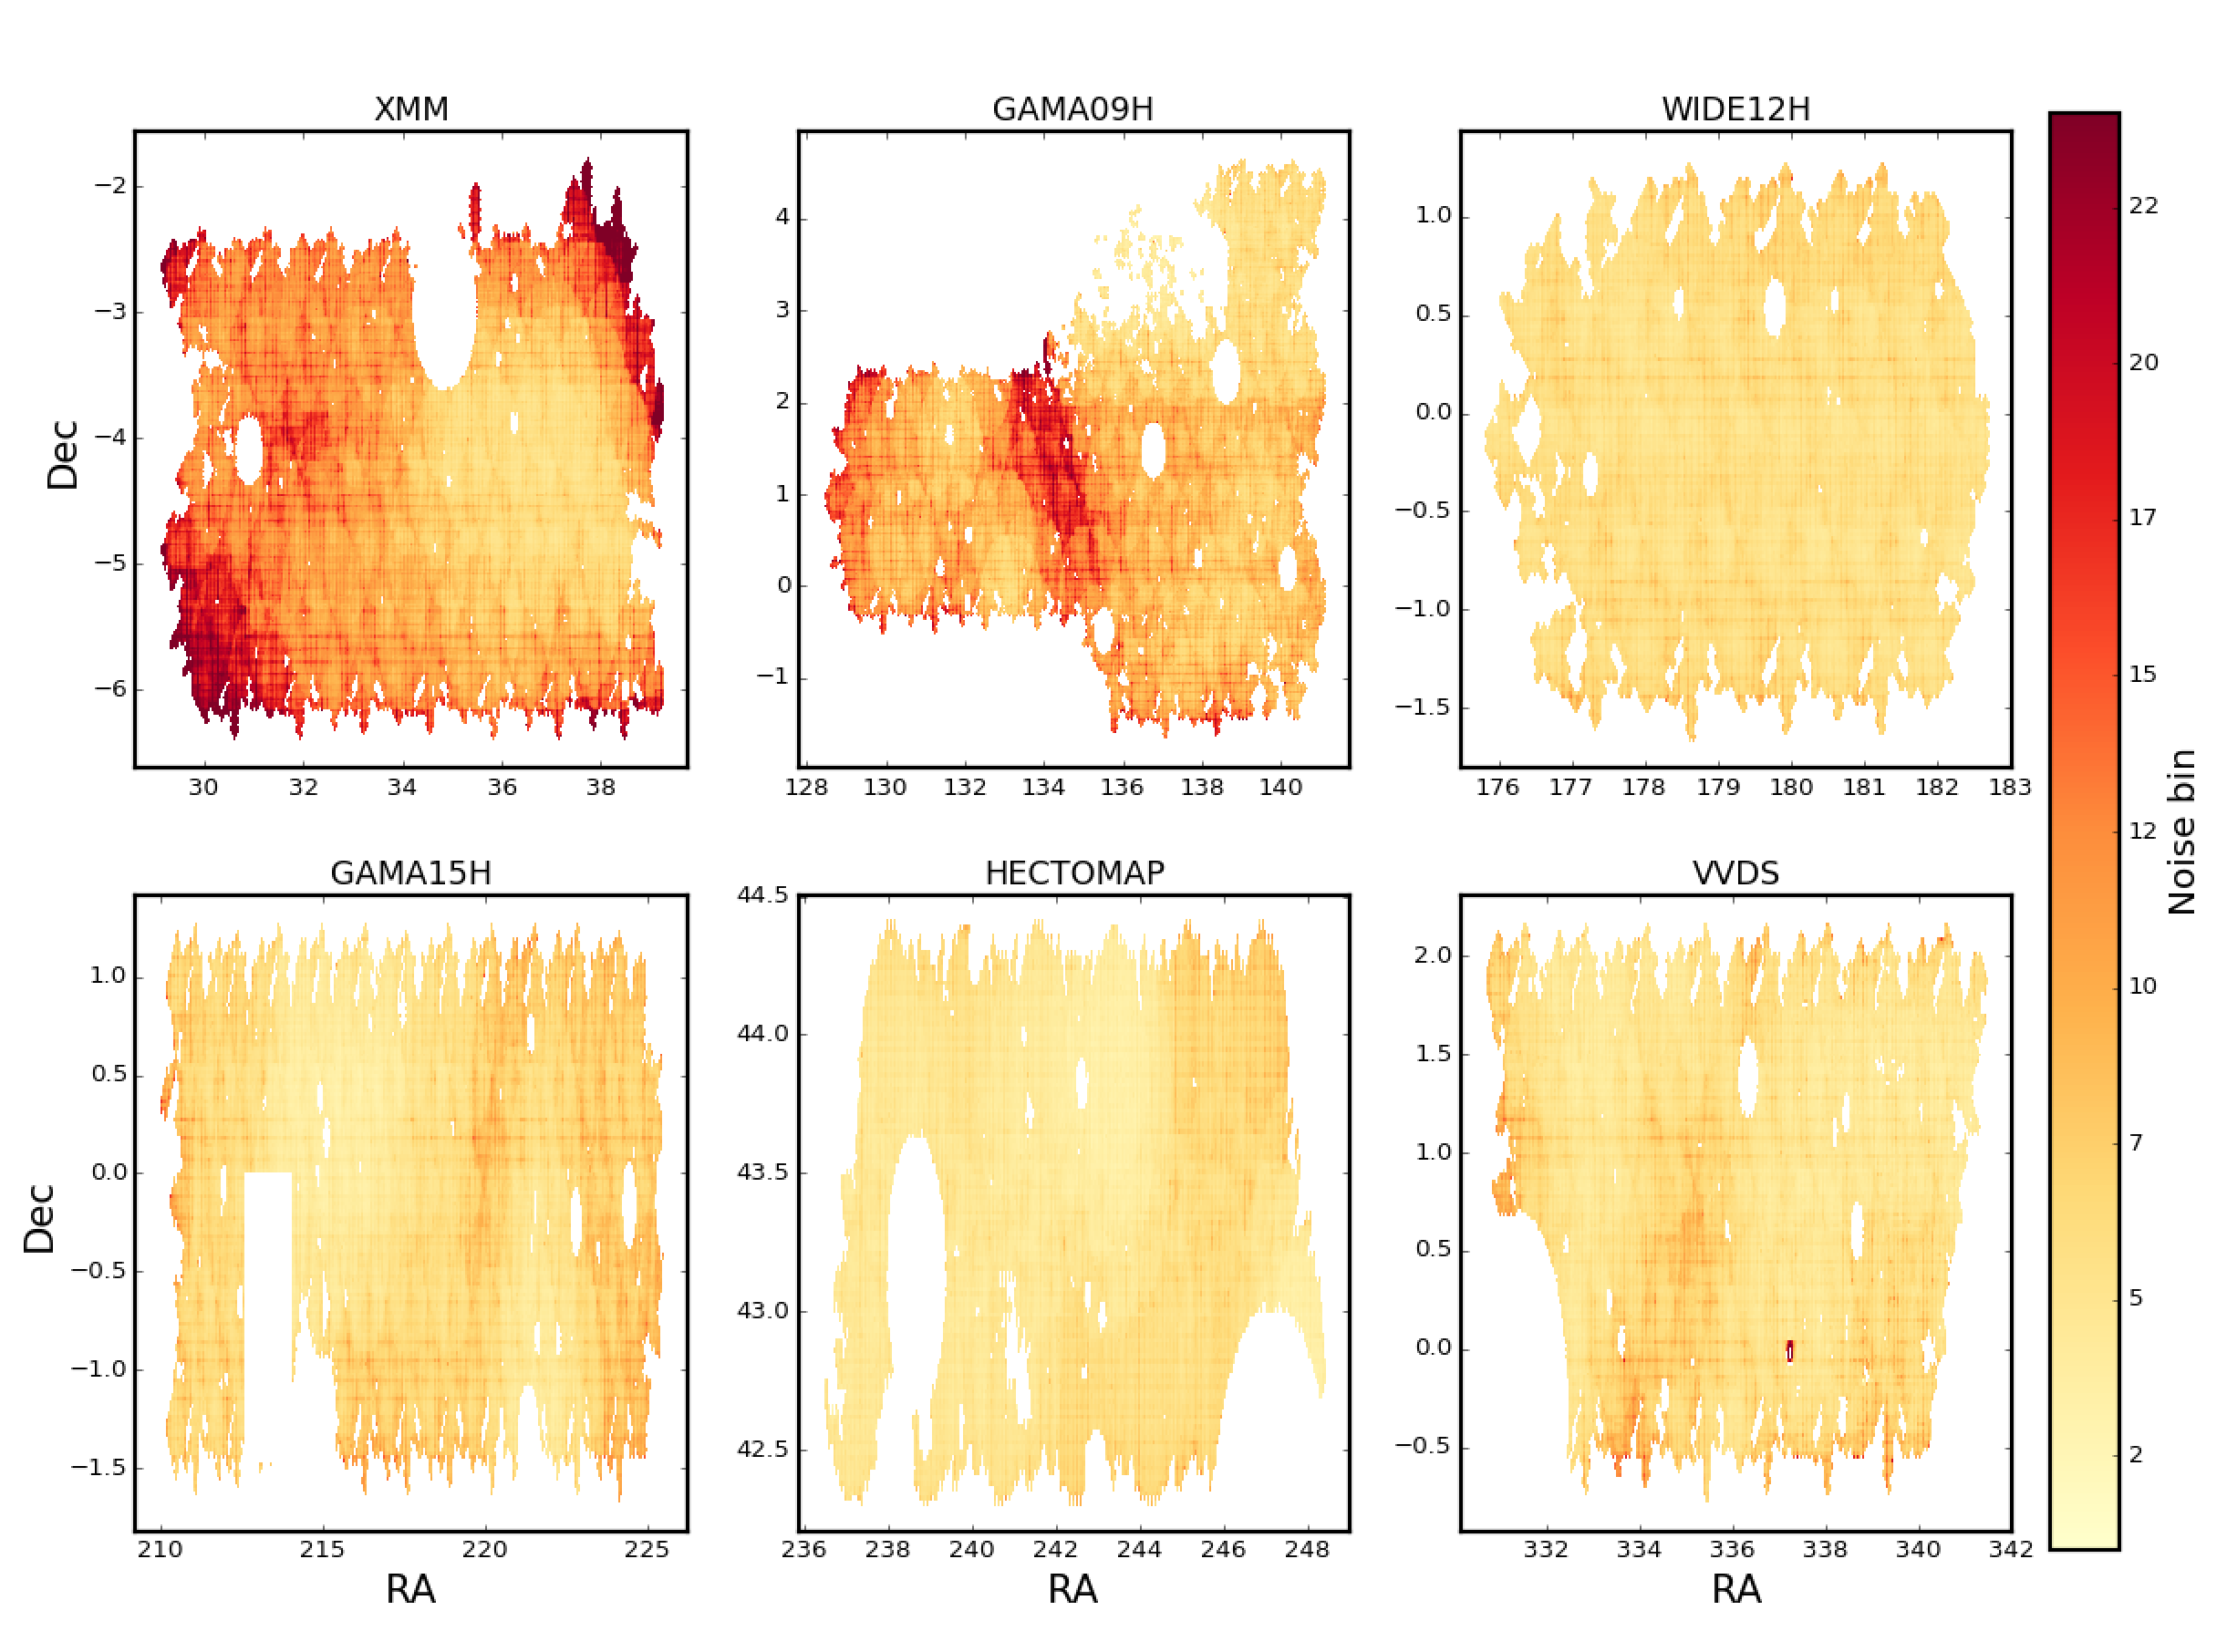
\includegraphics[width=\textwidth]{radec_noise_bin.png}
    \caption{
       The distribution of the flux variance bin (from 1-23) as a function of position for the six different observed regions.
    }
    \label{fig:radec_noise_bin}
\end{figure*}


We further divide each flux variance bin into two bins based on flux. The low flux bin uses a fixed 24.6 minimum magnitude cut and a maximum magnitude defined by $S/N$<40.  For this lowest bin, we do not need to introduce additional measurement noise.  In the high flux bin we use the selection of $40<S/N<80$. We add additional measurement noise by a factor of 2 for these objects and modify the moment covariance matrix appropriately, allowing a sufficient number of prior galaxies to overlap.  Figure \ref{fig:sn_var} shows the number of objects as a function of flux variance and flux $S/N$ where we have drawn boxes around the different cuts.  Again, we build a separate of prior galaxies for each box.  Figure \ref{fig:miss_gal} shows the number of galaxies that we miss by using these cuts.  We also highlight the additional number of galaxies available at low $S/N$ once we trust the photo-zs at faint magnitudes.

\begin{figure}
    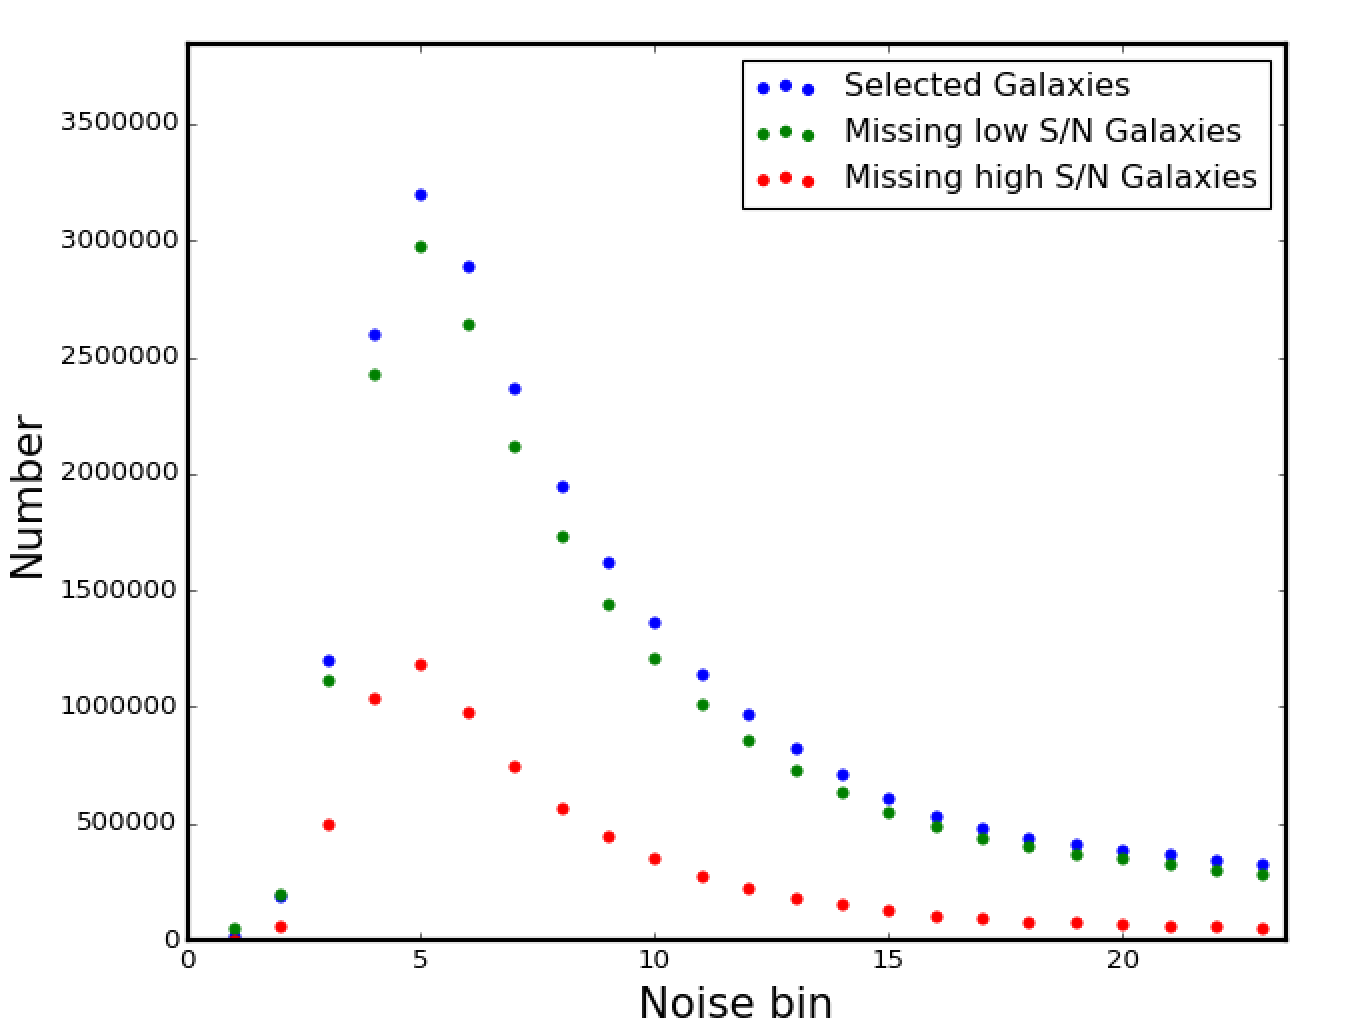
\includegraphics[width=0.5\textwidth]{miss_gal.png}
    \caption{
       The green points show the number of objects that we select as a function of noise bin.  The blue points show the low $S/N$ objects we cut in the current analyses, but still and have $S/N$>5 and thus are still potentially useful.  The red points show the high $S/N$ objects with  $S/N$ > 80.  These could also be potentially recovered by adding another set of priors with more additional noise, but was not done for this analysis. 
    }
    \label{fig:miss_gal}
\end{figure}

\begin{figure}
    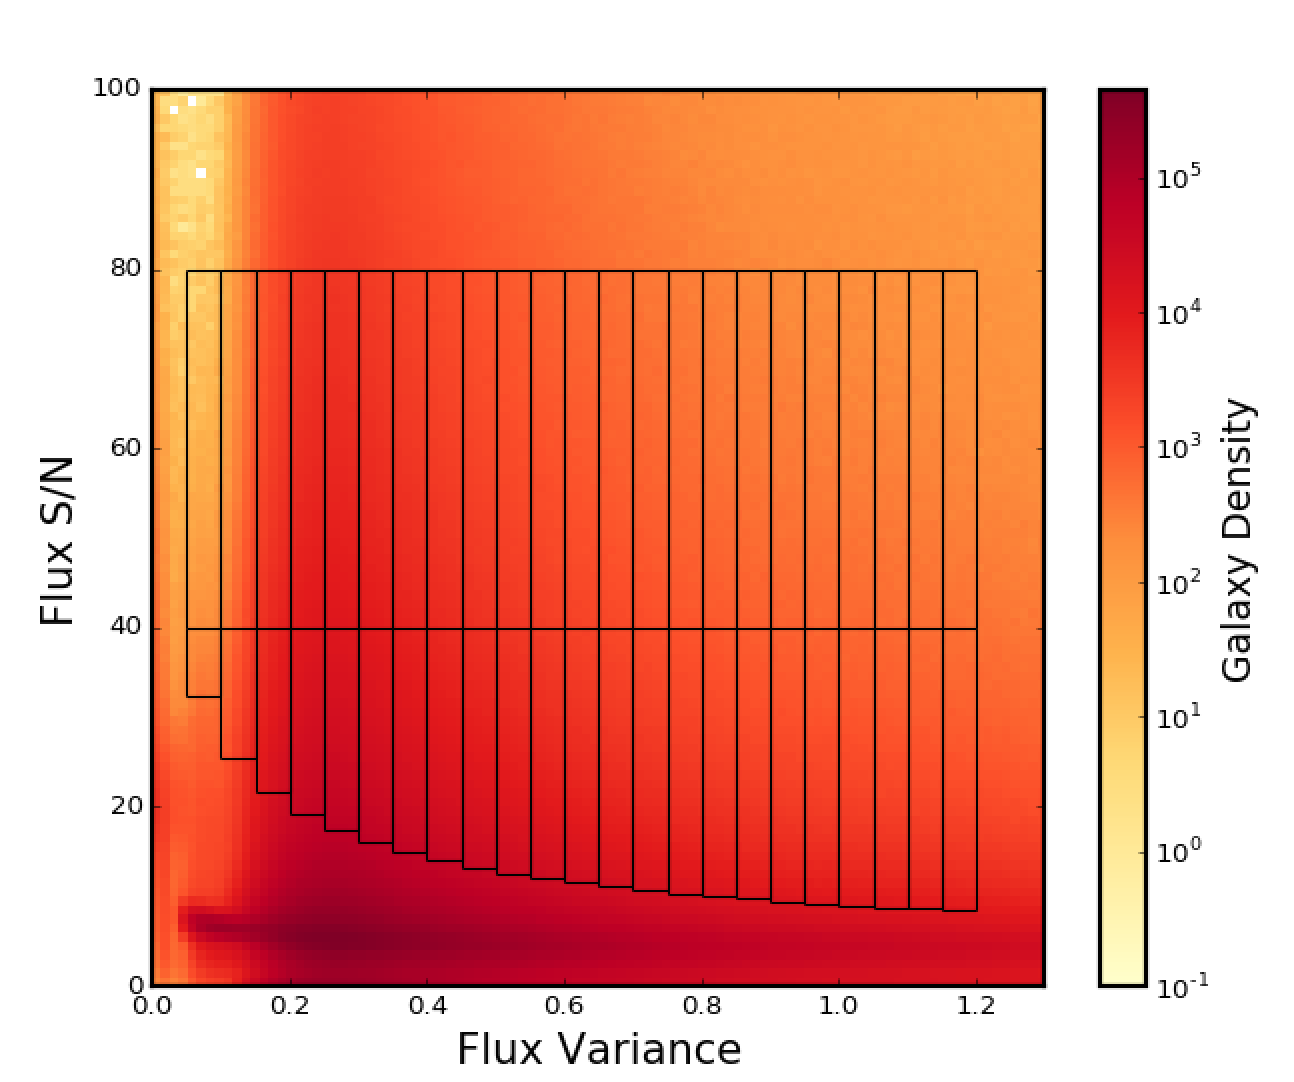
\includegraphics[width=0.5\textwidth]{sn_var.png}
    \caption{
       The number of galaxies that we select as a function of $S/N$ x-axis and flux variance y-axis.  The boxes indicated the galaxies targeted for this analysis.  We build a separate set of priors for each box.
    }
    \label{fig:sn_var}
\end{figure}


\section{Building the Prior}
\label{Sec:Prior}


\subsection{Deep Observations in HSC}
As part of the HSC survey, we observe two Ultra-Deep fields covering 4 deg$^2$.  One is centered on the COSMOS \citep{2007ApJS..172..196K} field while the other is in the SXDS \citep{SXDS} region.  In addition, there are four Deep regions covering 38 deg$^2$.  The 5 $\sigma$ point source depths of the observed Ultra-Deep and Deep fields are 27.2 and 26.5 respectively in the $i$-band \cite{DataPaper:inprep}.  For this data release, the Ultra-Deep fields have $\sim$6 times the exposure time of the wide field observations, matching the difference between the peaks in the flux variance distribution as shown in  Figure \ref{fig:flux_var}.  In \cite{Bernstein2016} (see Figure 3), we show that this is sufficiently deep so as to not introduce a significant bias due to the fact that the templates are noisy.  Ultimately, the Ultra-Deep fields will go to a depth of 27.7 in the $i$-band which will be more than sufficient.  We can also potentially use the Deep data at that point because it will have reached roughly the same depth, 27.1, as the current Ultra-Deep data.  Therefore, we can use the observed Ultra-Deep data to construct the distribution of true moments $P(\vecM_{\rm true}|g)$. 

In Figure \ref{fig:cosmos_sxds_bin4} we show a comparison of the moments from the two Ultra-Deep fields.  For easier comparison we show the flux, normalized size and ellipticities instead of the unnormalized moments.  The normalized size is defined as $M_r/M_f$ and $E1=M_+/M_r$ and $E2=M_\times/M_r$.  These comparisons do not include the 24.6 magnitude cut or the requirement of a detection on the wide-depth stack.  Instead, we reduce the minimum cut to $S/N_{\rm min}=5$ for the lowest flux bin to see any possible deviations over the whole flux range.  They are in excellent agreement.  We do not show the moment derivatives w.r.t. to shear, but they agree well also. Because of the observed agreement we restrict ourselves to using data from the COSMIS field.

\begin{figure*}
    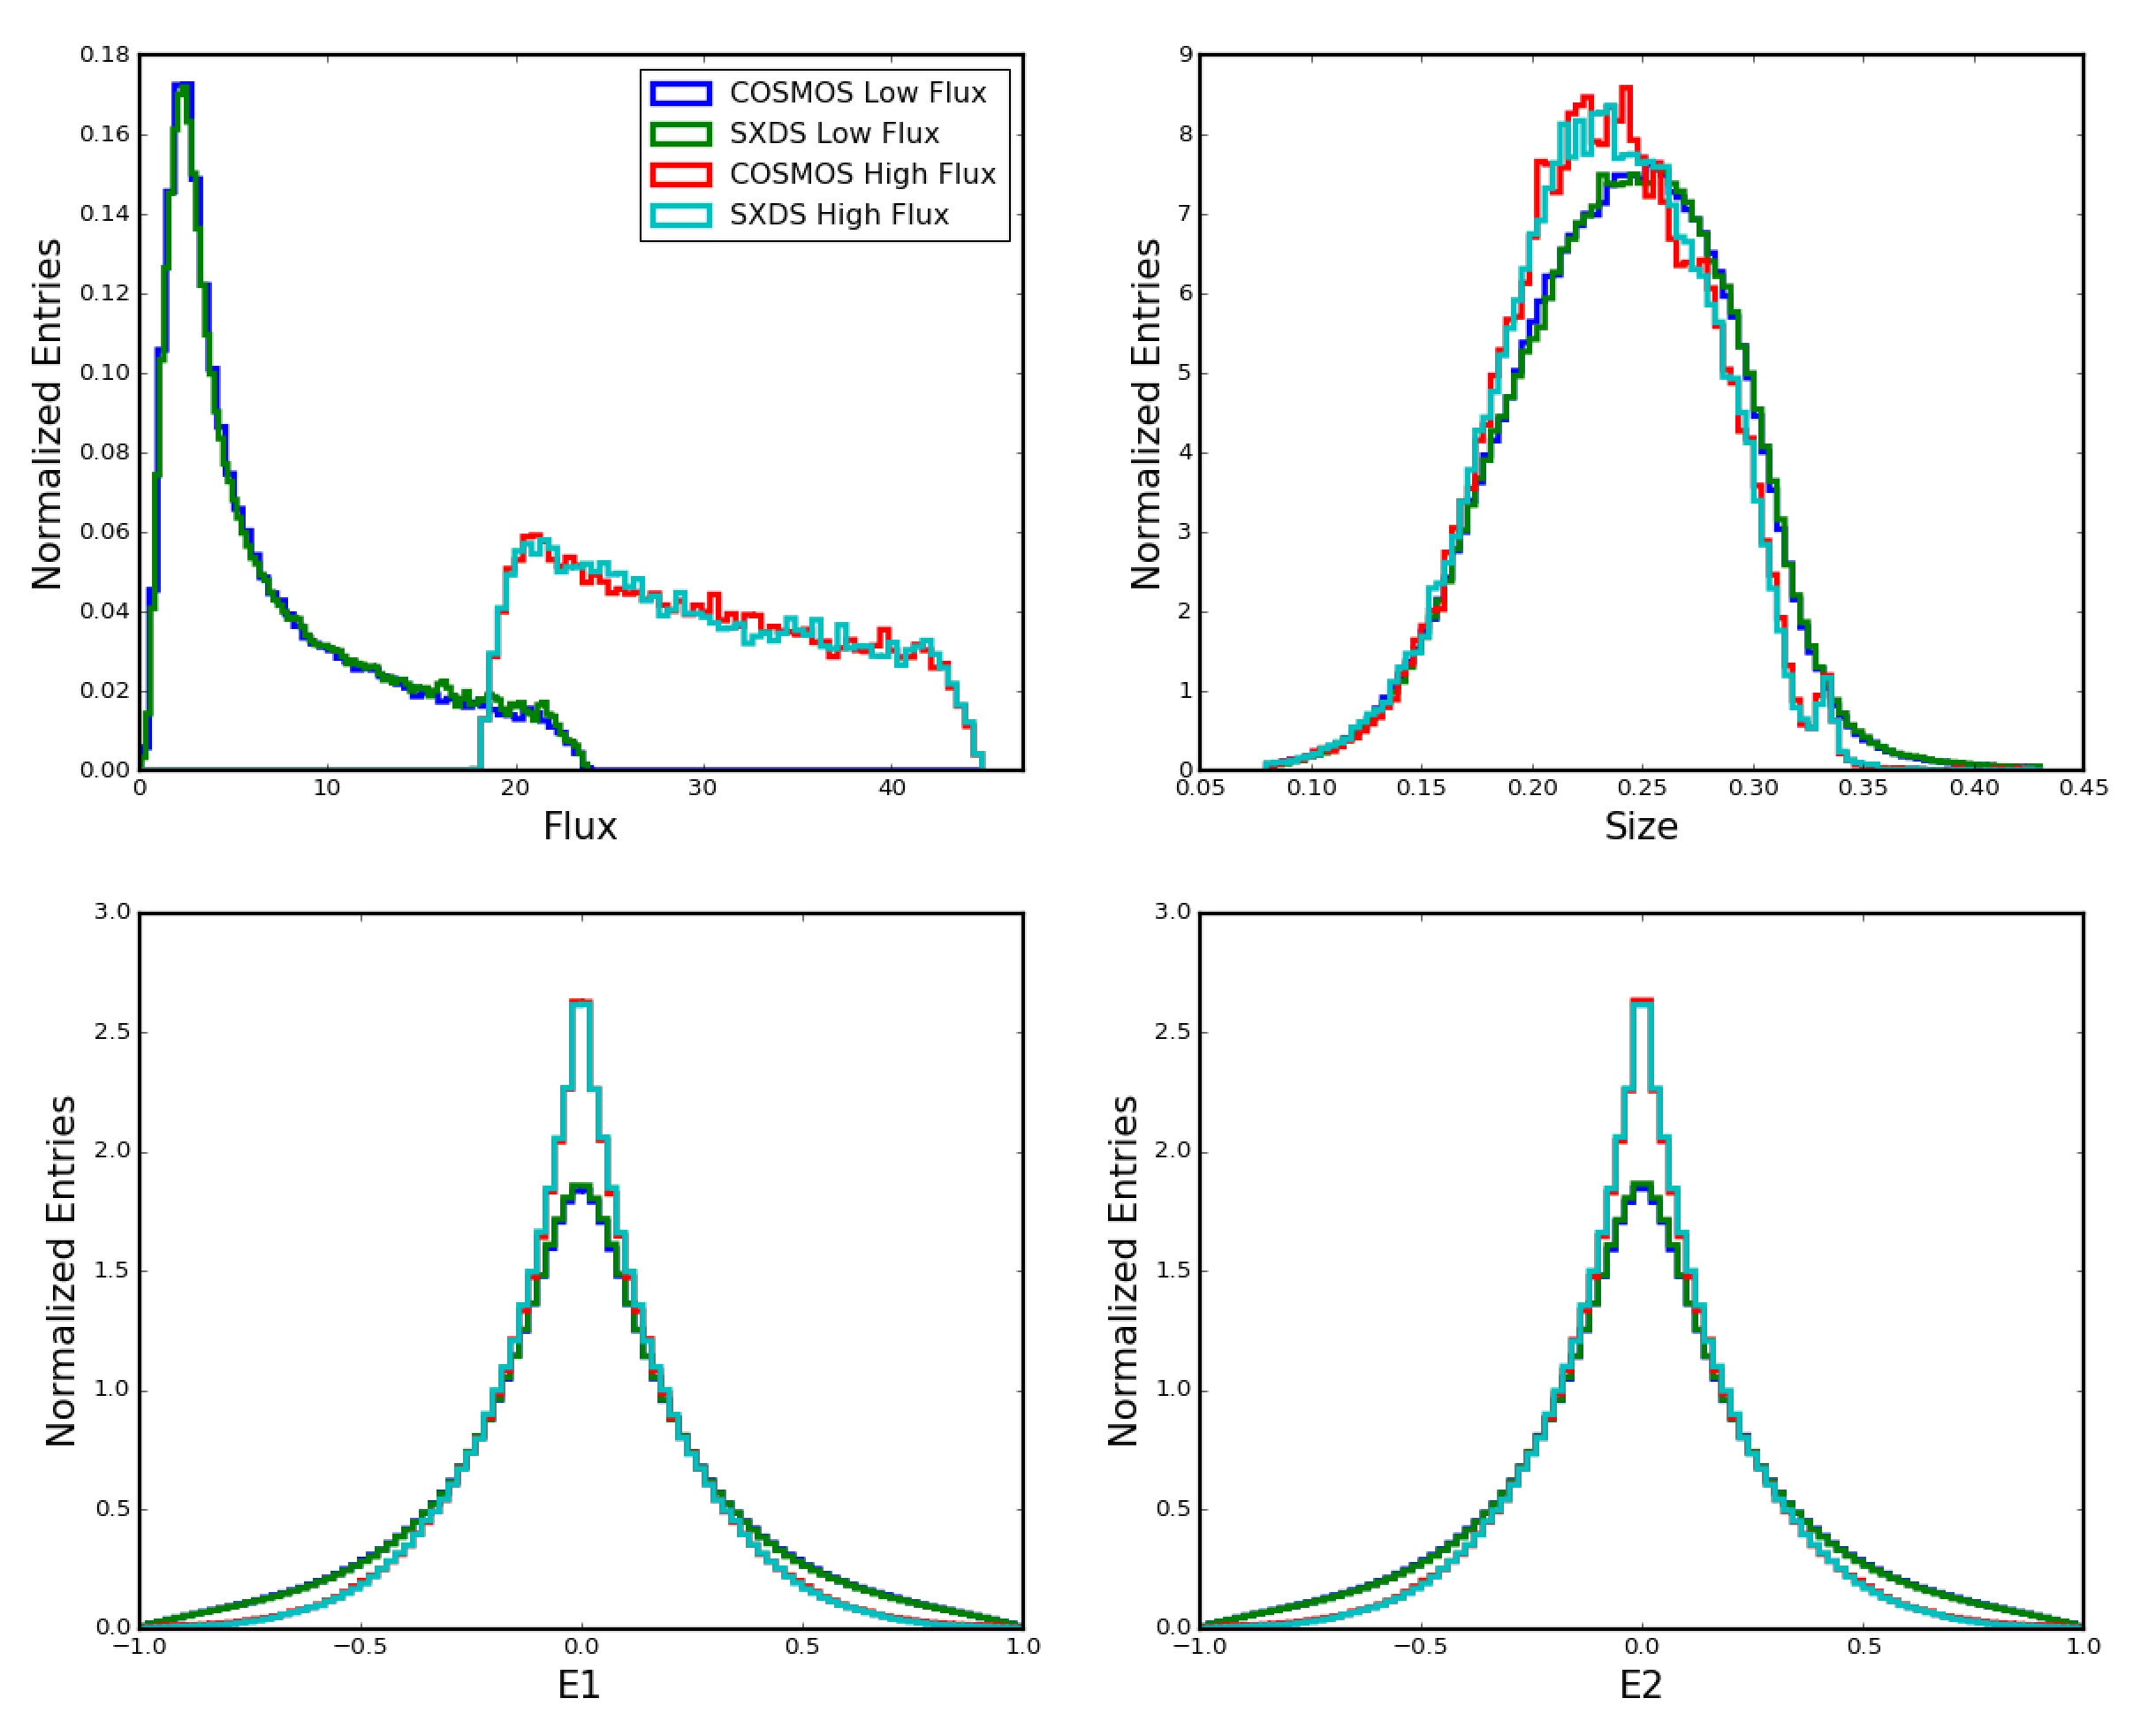
\includegraphics[width=\textwidth]{cosmos_sxds_bin4.png}
    \caption{
       Distribution of moments for the low and high flux bin for COSMOS and SXDS.
    }
    \label{fig:cosmos_sxds_bin4}
\end{figure*}


A key assumption in our method is that the deep data used to build the prior is truly representative of the shallower, wide-field observations.  There are a number of factors that would cause this to be untrue:  
\begin{itemize}
\item The deeper data will extend to higher redshift, potentially probing a different population of galaxies.
\item Selecting subsets of the wide field data based on flux, size, color, photo-z, or photo-z quality may change the underlying prior.  
\item Blending could potentially be different in the lower noise deep data.
\end{itemize}
After describing the observed deep data in HSC, we will try to address each of these concerns.

\subsection{Different Galaxy Populations}
To reduce the impact of potentially different redshift populations between the deep and wide-field data, we make use of the wide-depth COSMOS stacks as described in \cite{DataPaper:inprep}.  These were combinations of visits in COSMOS chosen to mimic the same observing time that we have in the wide-field.  We use the sample with the best seeing (FWHM $\sim 0.5$\arcsec), because there was an identified problem with the median seeing stack and the worst seeing stack had seeing (FWHM $\sim$ 1\arcsec) very different than the nominal wide-field observations.  These are used to reject objects from the prior that would not be detected in the wide-field data.  By doing this, we do miss detections below the wide-depth stack detection limit, but with our magnitude cut at 24.6 this is not a big effect because we are well above the detection limit.

\subsection{Analyses Cuts}
Ideally, we would not need a different prior for each set of cuts that is applied to the data.  In this section we examine common cuts that are made and how this changes the resulting priors.
\subsubsection{Redshift evolution}
We have photo-z estimates for every galaxy in the Ultra-Deep fields \citep{Photoz:inprep,Speagle:inprep}.  Furthermore, the COSMOS field is essential for training/testing the photo-z algorithms because of the many ancillary data available. We can therefore see how the moments of the prior objects change as a function of photo-z.  Figure \ref{fig:z_prior_moments} shows the change in the normalized moments for different redshift slices.  We use the FrankenZ photo-z estimator \cite{Speagle:inprep}, but the trends are not sensitive to the particular choice of photo-z estimator. This plot shows that, as expected, higher redshift objects are smaller, noisier, and fainter.  The problem here is that when selecting background galaxies for weak lensing analyses, we will target a specific redshift range behind the lenses that will not match the redshift distribution of the prior galaxies.  As stated in ~\cite{Bernstein2016}, the best solution is to jointly infer both the redshift and shear.  However, for this analysis we choose a simpler solution.  Since a majority of interesting lenses lie below redshift $\sim0.7$, we re-weight each prior galaxy with the fraction of its photo-z pdf above redshift 0.7.

\begin{figure*}
    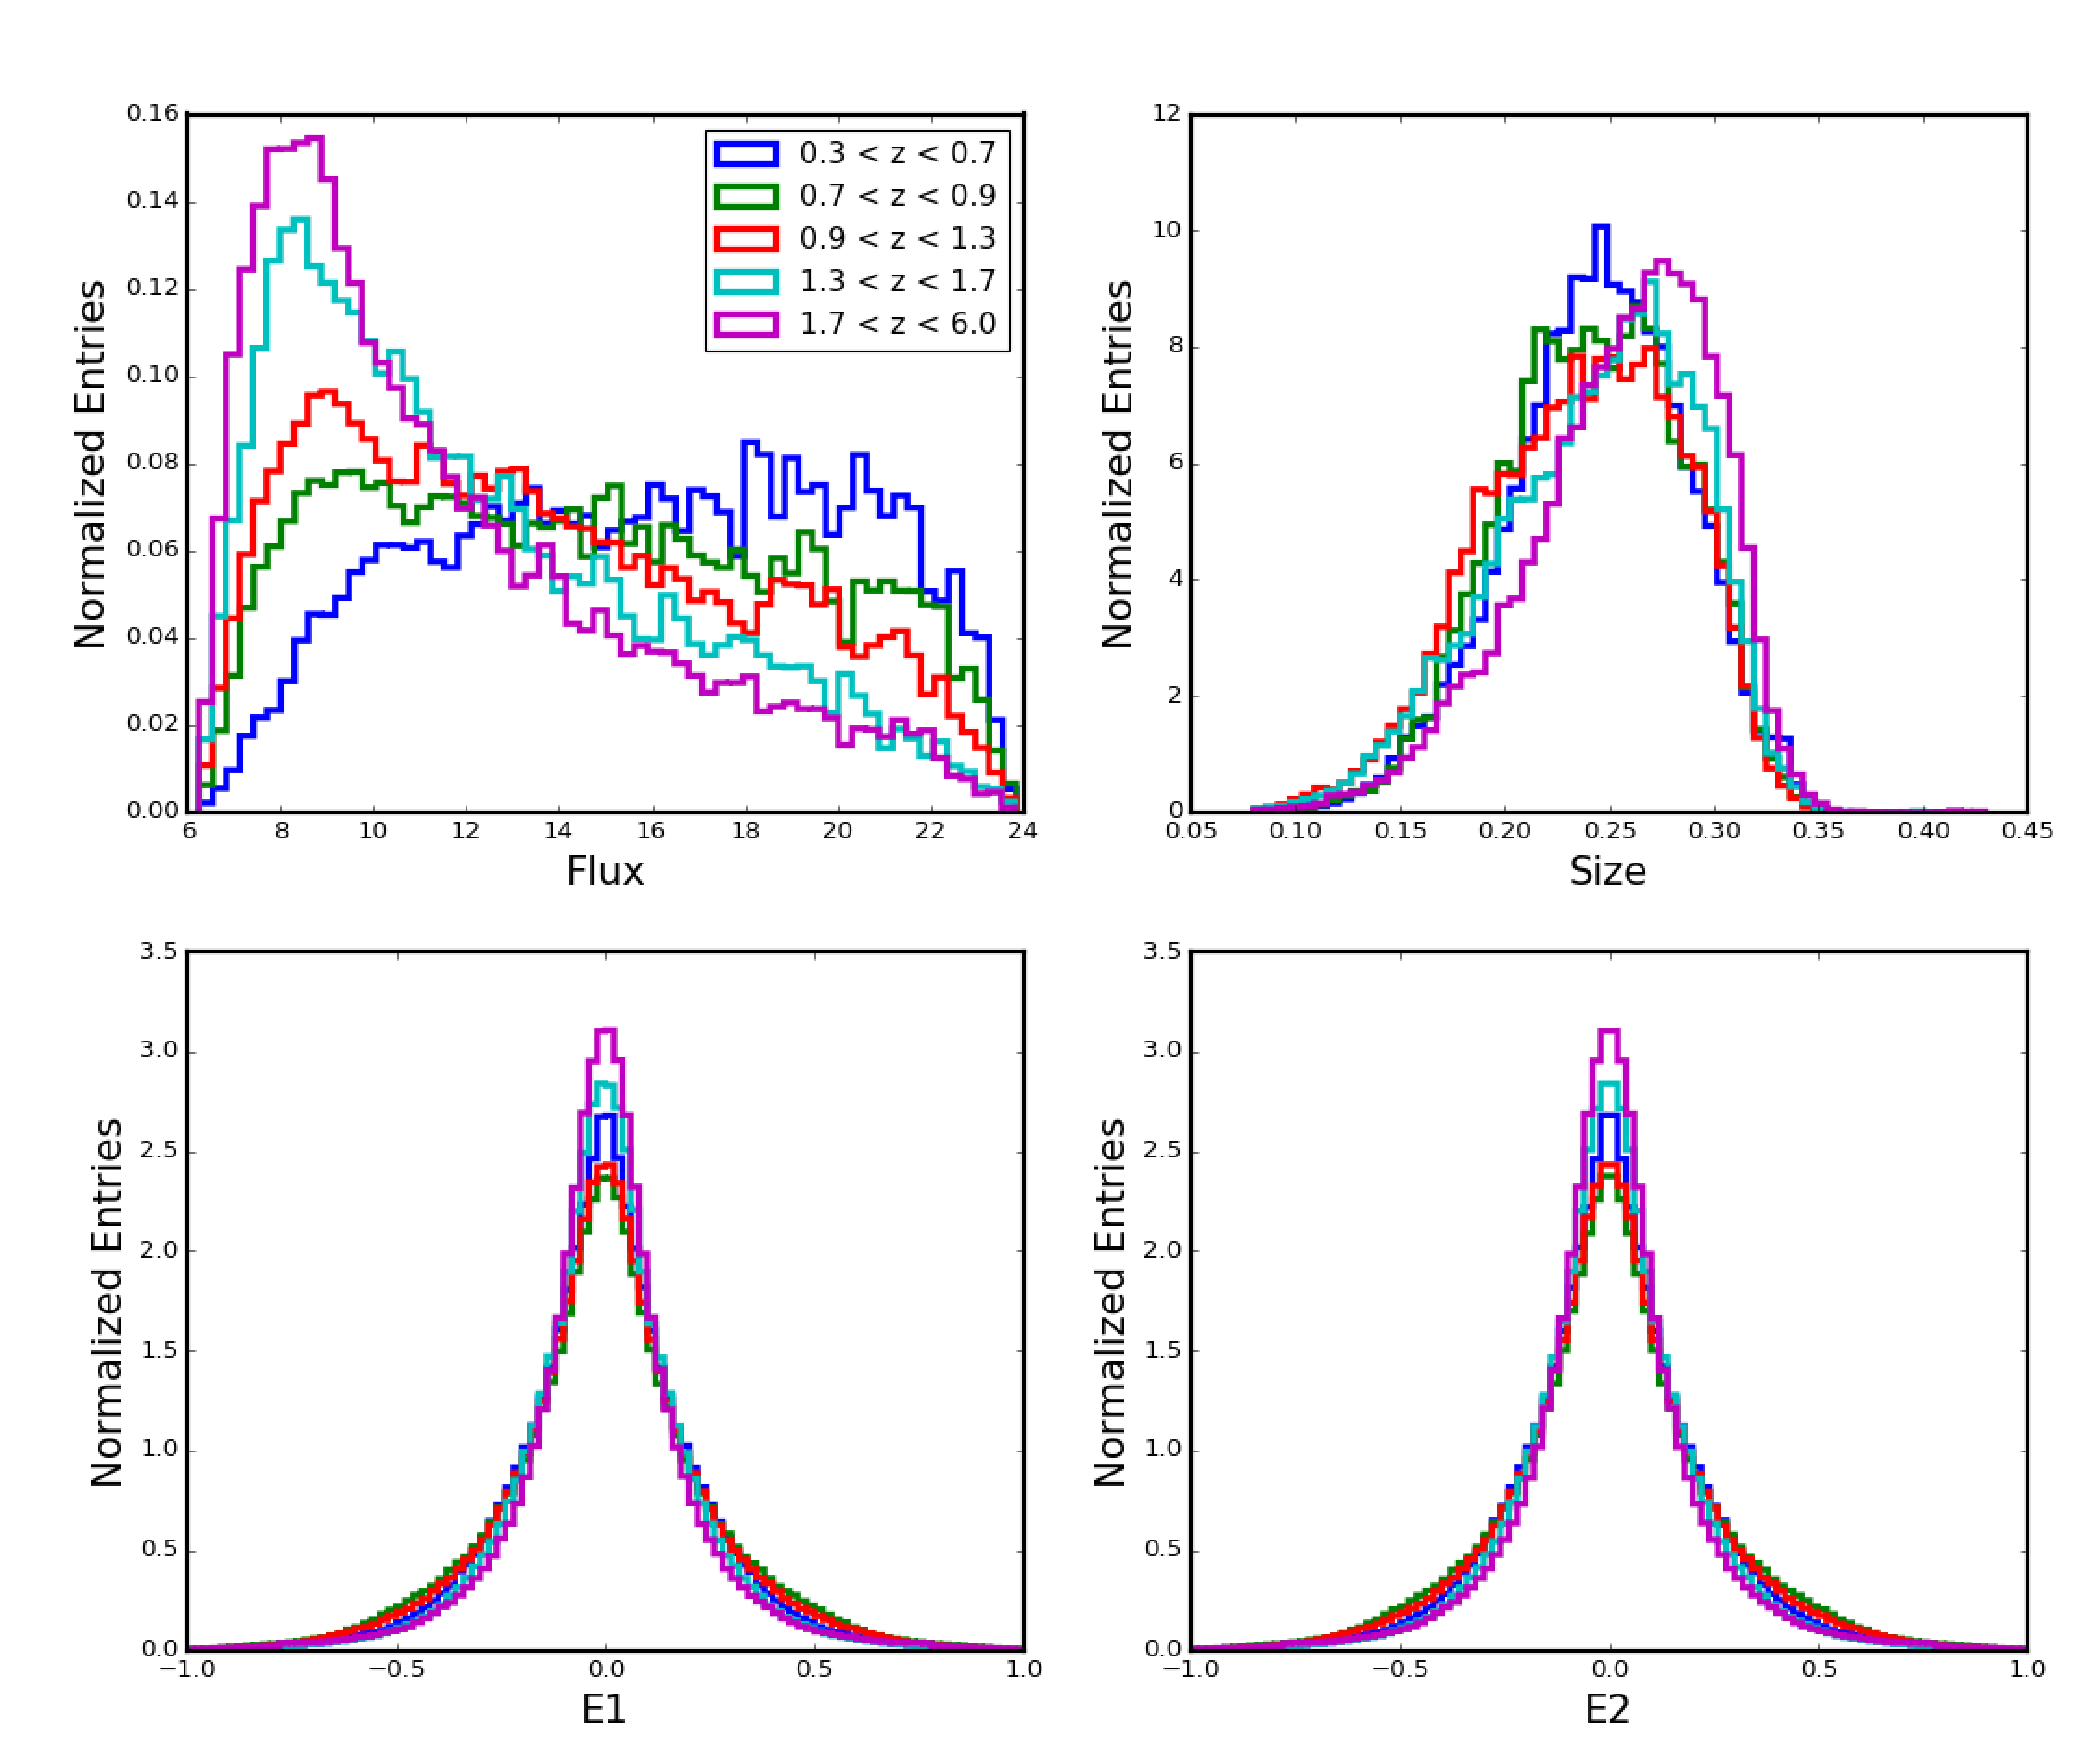
\includegraphics[width=\textwidth]{z_prior_moments.png}
    \caption{
       Normalized Moment distributions for different redshift slices for the low flux and fifth noise bin.  The size in the top right is defined as $M_r/M_f$.  This size is measured in the Fourier domain, so small values correspond to large objects.  The E1 and E2 values in the lower panels are defined as $M_+/M_r$ and $M_\times/M_r$ respectively.
    }
    \label{fig:z_prior_moments}
\end{figure*}

\subsubsection{Photo-z quality}

If we apply cuts on the photo-z quality in the wide-field data this can potentially lead to differences from the prior.  Photo-z algorithms will typically fail on the fainter, smaller galaxies.  To test the impact of this, we applied three different quality cuts from the FrankenZ photo-z catalogs of the COSMOS field.  These cuts correspond to cutting out the poorest measured 10, 40 and 60 $\%$ of the data.   We found that applying the first cut to our prior objects had no discernible change in the moment distributions.  In contrast, the third cut had quite a significant impact.  The second cut had only moderate affect which is shown below.  Part of the reason cutting out such a large fraction of the data does not have a big impact is because we are already excluding the faintest objects.

For comparison we create a sample based on the second quality cut that is also weighted by the fraction of the pdf $\geq 0.7$



\subsubsection{Color-Color cuts}
An alternative method to using photo-zs is to select background galaxies by using cuts in color-color space.  The cuts are judiciously chosen to remove galaxies at unwanted redshift.  In \cite{ClusterSel:inprep} a comparison is done on the difference between these two methods as applied to 1st-year HSC data.  In order to use such a selection we need to see how the prior distrubtion is changed by these cuts.  We tested this by only selecting prior objects that satisfied the set of low redshift color-color cuts as described in Appendix 1 of ~\citep{ClusterSel:inprep}.  We use both the red and blue galaxy samples from these cuts.   As can be seen below, the color cut selection produces prior distributions that are almost equivalent to the FrankenZ $\le 0.7$ results.



\subsubsection{Comparisons}

We estimate the impact that each of the previous cuts has on the prior distributions.  In Figure \ref{fig:diff_flux_prior},  we compare the flux distribution for two different noise bins from the low flux region.  We only show the flux, because the other moments and derivatives had little or no change with the different cuts.  Specifically, we create different priors with:
\begin{itemize}
\item Weight each prior object by the fraction of FrankenZ pdf $\ge 0.7$.
\item Weight each prior object by the fraction of MLZ pdf $\ge 0.7$.
\item Apply the second FrankzenZ photo-z quality cut and weight by the fraction of FrankenZ pdf $\ge 0.7$.
\item Color cut selection
\end{itemize}
From the figure we see that the main effect is to change the relative number of objects at low and high flux values. The maximum deviations show $\pm 15\%$ changes in the peak.  In Section \ref{Sec:Data:Priors} we compare the shear signal using catalogs created from the different priors that have the maximum deviation.  These show no significant differences in the shear signal.  Given these results, we conclude that for the first year weak lensing sciences we should be able to use a nominal prior set and still be able to use different photo-z estimators, make moderate cuts on photo-z quality or use color-color cuts without a significant impact.  In the future, with more data, this will likely no longer be the case.

\begin{figure*}
    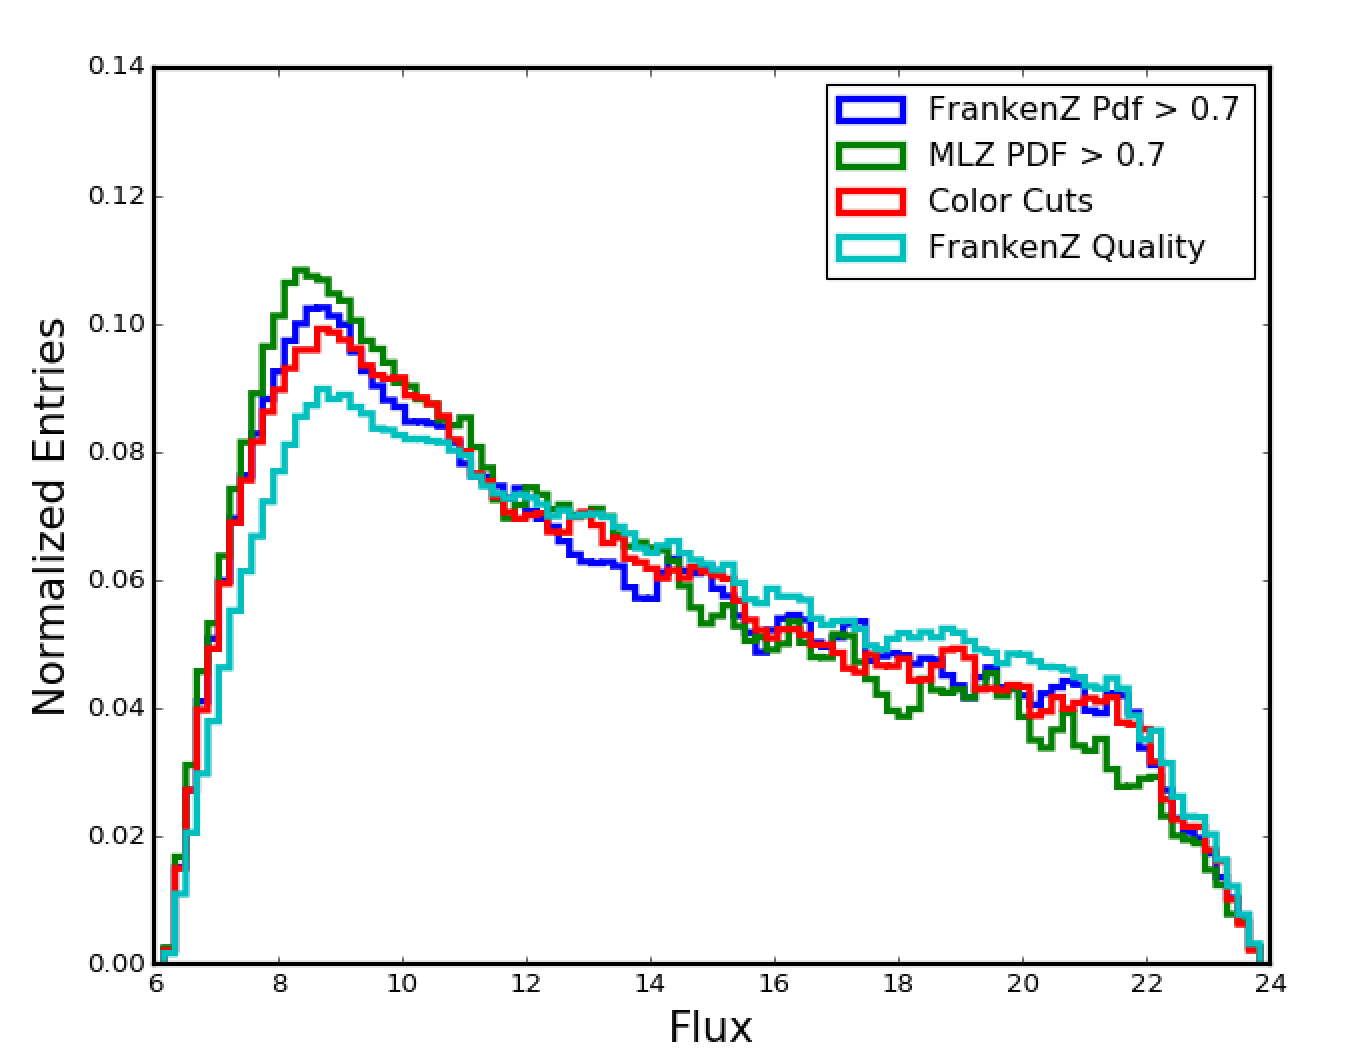
\includegraphics[width=0.48\textwidth]{diff_flux_prior_bin4.png}
    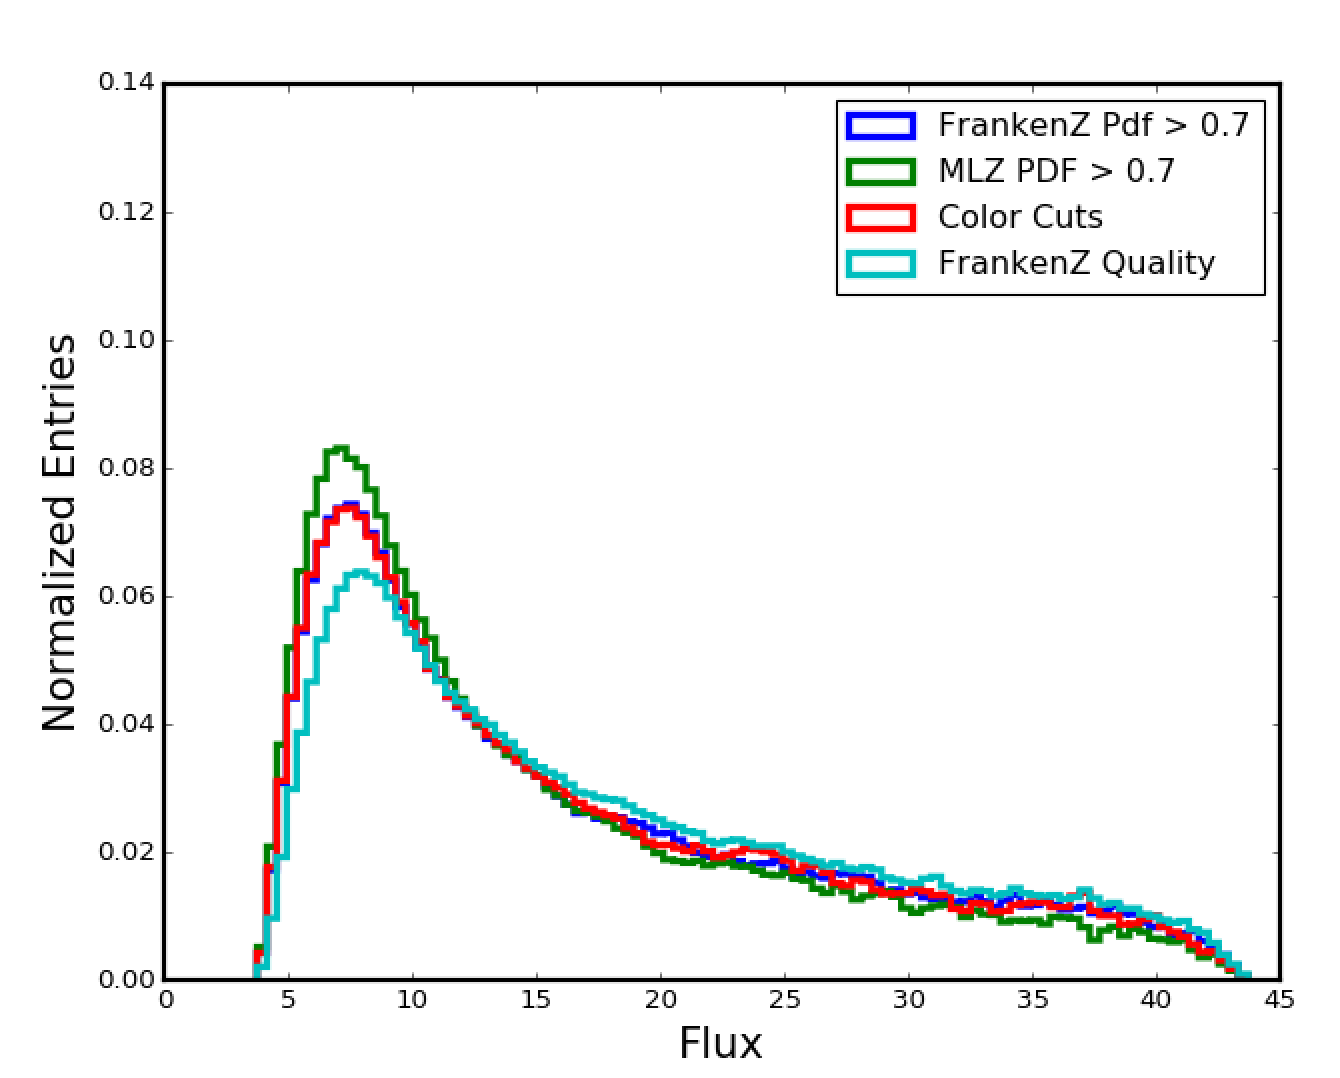
\includegraphics[width=0.48\textwidth]{diff_flux_prior_bin17.png}
    \caption{
       Changes in the distribution of the flux moment of the prior galaxies with four different selections: weighing each prior galaxy with the fraction of the photo-z pdf above 0.7 for the FrankenZ and MLZ photo-z estimates.  On the left are the prior galaxies in the fifth noise bin and on the right are the prior galaxies from the 17th noise bin.
    }
    \label{fig:diff_flux_prior}
\end{figure*}



\subsection{Blending}
Because of the inherent challenge of deblending deep optical images and knowing that the HSC software had significant problems in crowded regions \citep{CatalogPaper:inprep}, we use simulations to test for possible biases that can occur from blending.  See Section \ref{Sec:SimsBlend} for a thorough treatment.

\subsection{Final selection of objects for prior}
Objects that are added to our priors must pass the following criteria:
\begin{itemize}
\item They must have a matched detection on the shallow wide-depth COSMOS observations.
\item Each object is weighted by the fraction of its photo-z pdf $> 0.7$.
\item The flux variance must be $< 0.15$. This is necessary to avoid noisy templates in the outer regions of the Ultra-Deep field.
\item The footprint area must be $< 10000$ pixels to reject large bright objects that can consume too much memory.
\item Randomly sample 40$\%$ of the galaxies to be included.
\item No cut on the an object's minimum size

\end{itemize}
Once a prior object is selected we also add rotated, parity-inverted and shifted copies as described in \cite{Bernstein2016}.  Typically, an object will have a multiplicity of a few hundred.

Because we make no cut on the size, stars are included in our prior objects in addition to galaxies.  You can see their presence as a bump in the normalized size distribution at $\sim 0.33$ for the high S/N sample in Figure \ref{fig:cosmos_sxds_bin4}.  This bump becomes more pronounced for the high flux and larger noise bins because the flux limit is higher in those samples.  These should have minimal impact on shear measurement if the stellar density observed in the wide fields is represented well by the COSMOS field.  Given that the galactic latitude is roughly the same for the COSMOS and wide-field this is not a problem.  Is this really true?


\section{Validation on Simulations}
\label{Sec:Sims}

We use the same suite of simulations as described in \cite{SimPaper:inprep} to validate and test the BFD method.  These simulations create a grid of 100x100 objects where all objects have the same applied shear.  The shear values for both components, $g_1$ and $g_2$, are randomly selected from the range -0.05 to 0.05.  For each image we choose the PSF and pixel noise from a randomly selected position in the coadded data.  We use the average pixel correlation as described in Sect ~\ref{Sec:Noise}. 
 
In \cite{SimPaper:inprep}, four different simulation sets are described.  Because we need to simulate an additional deeper set of galaxies, we can only use the simulations based on the parametric fits to the COSMOS galaxies for validation.  This corresponds to sample 2.  As stated in \cite{SimPaper:inprep}, after processing the parametric galaxies through the HSC pipeline, we found that the observed properties did not quite match those in the HSC data.  This was attributed to the fact that the parametric fits were done on masked HST images and were excluding things like nearby light and contamination from neighbors. This problem was remedied by using real galaxy images from HST, without any blending and object masks from HSC.  However, we cannot currently use these simulations for BFD processing.  
Since we are not using these simulations to derive calibration factors, it is not as critical that the simulations match the data, only that the observed distributions are roughly correct.

For our validation tests, we chose to use 30 deep images simulated with $10\%$ of the average HSC pixel noise, which is close to the increased depth of the Ultra-Deep fields relative to the wide data.   We simulated 800 images and processed them with the BFD code in the same manner as the HSC data.  Some fraction of these images had selected pixel noise and PSF such that the flux variance was outside of our chosen range.  These images were ignored.  There were also not any images in the two lowest flux variance bins so they were not used.  

We measured shear using two different sets of flux selection cuts.  The first was to use the full $S/N$ range from $5 < S/N < 80$, while the second was to match the magnitude cuts we used in the HSC data and is labeled "24.6 Cut".  For both cuts we divide the data into a low and high flux group based on if the $S/N$ is less than or greater than 40.  To find the multiplicative and additive biases we computed the average shear for each image and then fit for the biases as a function of input true shear.  Table \ref{table:sim_bias} summarizes the resulting biases for the different selection cuts.  An additional cross check is to compute the shear based on the low or high flux priors alone and compare the result.  All biases are consistent with zero.

\begin{table}
\caption{Measured Biases on Simulations}\label{table:sim_bias}
\begin{center}
\begin{tabular}{lcc}
\hline
Sample & Multiplicative Bias & Additive Bias \\ \hline \hline
Full Range           & 0.6 $\pm$ 0.3 $\%$& -$2.0$ $\pm$ $1\times10^{-4}$ \\
Full Range Low Flux  & 0.8 $\pm$ 0.3 $\%$& -$2.0$ $\pm$ $1\times10^{-4}$ \\
Full Range High Flux & 0.4 $\pm$ 0.7 $\%$&  $2.0$ $\pm$ $2\times10^{-4}$ \\
24.6 Cut             & 0.1 $\pm$ 0.3 $\%$& -$0.6$ $\pm$ $1\times10^{-4}$ \\
24.6 Cut Low Flux    & 0.1 $\pm$ 0.5 $\%$&  $0.7$ $\pm$ $1\times10^{-4}$ \\
24.6 Cut High Flux   & 1.0 $\pm$ 0.7 $\%$&  $4.0$ $\pm$ $2\times10^{-4}$ \\
\hline
\end{tabular}
\end{center}
\end{table}

In addition, we used the simulations to validate and optimize some of the parameters.  We tested the following parameters:
\begin{itemize}
\item The adding of 2x noise to the higher prior flux bin was enough to reduce the bias in the high $S/N$ regime.
\item Choice of how fine to bin the flux variance for creating different priors.  The chosen bin width was 0.05.  Relaxing this to 0.1 introduced a $1\%$ bias in the shear.
\item Ignoring the pixel correlations introduced a $\sim 3\%$ bias.
\end{itemize}

\subsection{Blending in the simulations}
\label{Sec:SimsBlend}
Another potential problem is that the simulations from parametric galaxies do not include any blending of objects since they are based on postage stamps that have had neighbors masked.  It is important to verify that the deblending algorithm currently in use does not introduce any bias.  To test this, we created additional simulations with galaxies randomly placed on the image instead of on a grid.  Both deep and wide-field images were processed with the HSC deblender \citep{PipelinePaper:inprep}.   We varied the density from 10,000 to 40,000 galaxies per image which is close the observed HSC density.  No bias was found, as long as the density of the deep and and wide-field images was the same.


\section{Validation on data}
\label{Sec:Data}

Because we don't have a full simulation suite it is difficult to accurately estimate the absolute effect of different systematics.  We therefore ensure that when changing different parameters, the lensing signal around known objects does not significantly change.

\subsection{Selection terms}
As shown in \cite{Bernstein2016}, to properly account for the probability of detection, selection and shearing of $N$ galaxies distributed via a Poisson distribution on the sky, we must add additional terms to Eqns. ~\ref{eqn:qtot} and ~\ref{eqn:rtot}. 

\begin{align}
\label{eqn:qtot_sel}
\vecQ_{\rm tot} & \equiv \sum_i   \frac{\vecQ_i}{P_i} - n\Omega \vecQ_{\rm sel}\\
\label{eqn:rtot_sel}
\matR_{\rm tot} & \equiv \sum_i \left(
   \frac{\vecQ_i\vecQ_i^T}{P_i^2} - \frac{\matR_i}{P_i}\right) + n\Omega \matR_{\rm sel}\\,
\end{align}

where $n$ is the total galaxy sky density, $\Omega$ is the sky area, and $\vecQ_{\rm sel}$, and $\matR_{rm sel}$ are the derivatives of the selection probability.  In this equation we have only kept the terms that explicitly depend on $\vecg$.

To properly account for the selection terms, we need the total galaxy density and corresponding selection probability.  Remember, however, that we don't have a single selection probability, but one for each noise bin that we have built the prior for.  To compute these, we divide the data into \texttt{HEALpix} pixels to approximate the geometry of the survey.   If the pixel resolution is not large enough then area will be missed because we only use the pixel centers and not partial pixels to represent the survey.  For most lensing analyses, a pixel resolution of \texttt{Nside}=8192 should be sufficient when restricted to moderately small scales.

The $\matR_{\rm sel}$, and $\vecQ_{\rm sel}$ terms can be found for each pixel on the sky by calculating the average noise of the objects within it and using the appropriate term from that noise bin. To not be affected by local density fluctuations, we use the average galaxy density for each noise bin.  Figure ~\ref{fig:ave_gal_hp} plots the total galaxy number density as a function of noise bin for all pixels.  We overlay a line with the mean relation.  This density is for all objects that have a successful moment measurement, not just those that satisfy our selection criteria.  This plot also shows that, for the lowest bin, the galaxy density does not increase as expected.  This likely points to some error in the calculation of the noise or some other problem with the data in these regions.  We ignore objects from this bin for the remainder of the paper.  Combining these terms with the pixel center, we can create an extra catalog to account for the probability of detecting $N$ galaxies given a fixed solid  area.  This catalog can then be added as another set of sources.


\begin{figure}
    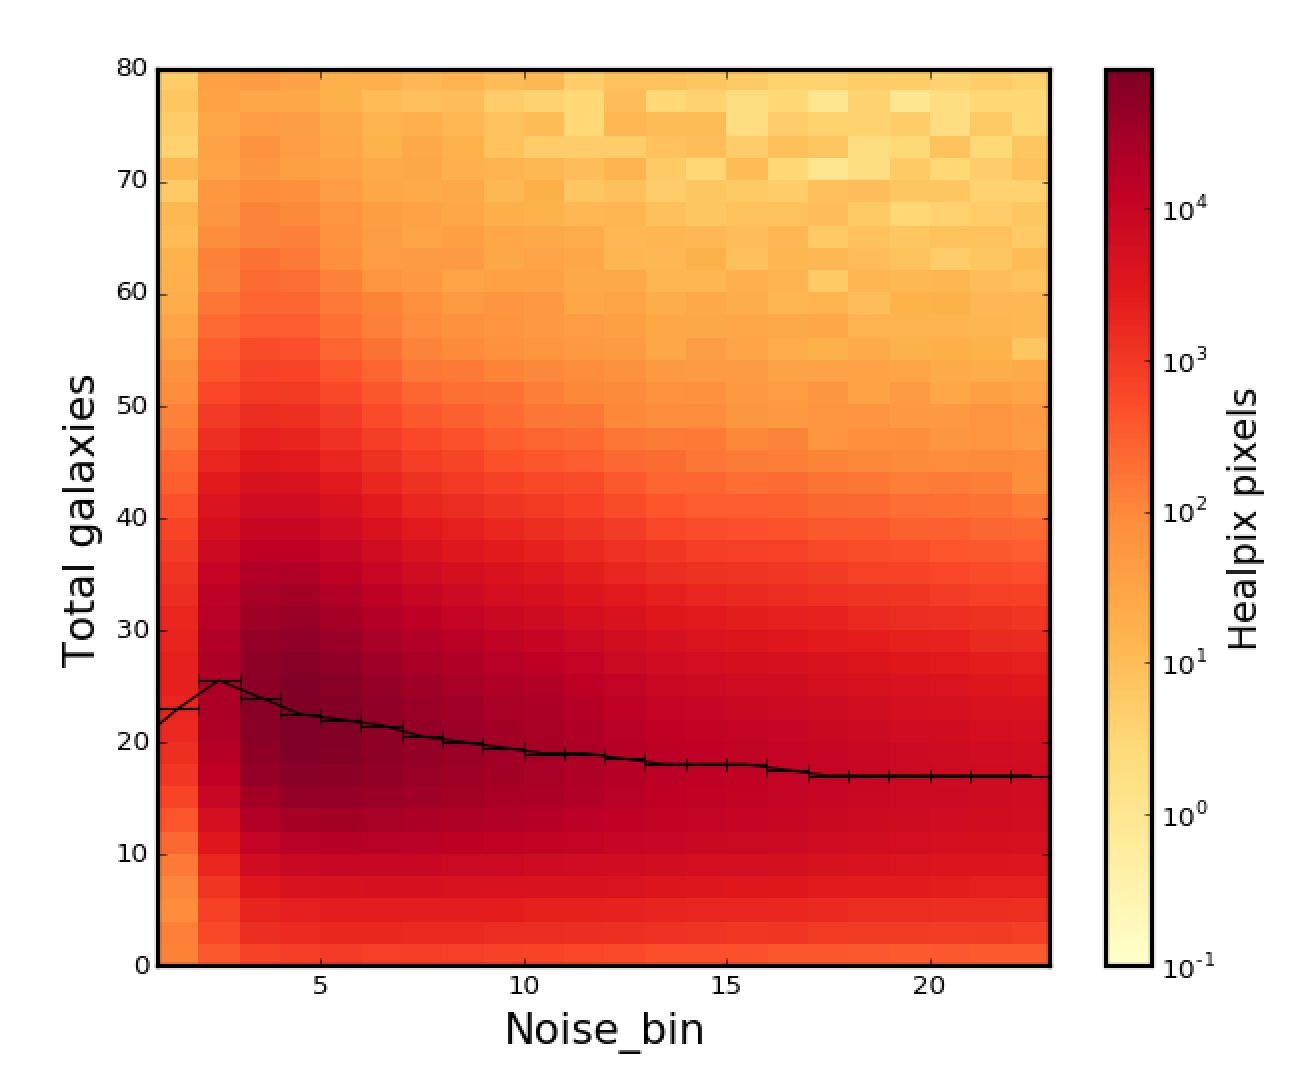
\includegraphics[width=0.5\textwidth]{ave_gal_hp.png}
    \caption{
    The total galaxy density vs. noise bin for \texttt{HEALpix} pixels of \texttt{Nside}=8192.  The black line shows the average over each noise bin.
    }
    \label{fig:ave_gal_hp}
\end{figure}

Given our selection cuts in this analyses, the impact of adding the selection terms typically results in $\sim 2-3\%$ corrections for stacked shear profiles.


\subsection{Tangential shear null tests}
If we stack the tangential shear around positions uncorrelated with the background galaxy shear these should result in zero shear.  We stack the average shear signal around the following three samples: star positions, random positions, and single visit centers.  This is shown in Figure \ref{fig:gt_null}.  For the star positions, we use the PSF stars on the coadd.  The visit centers correspond to all of the $i$-band visits.  All of these are consistent with zero.
\begin{figure*}
    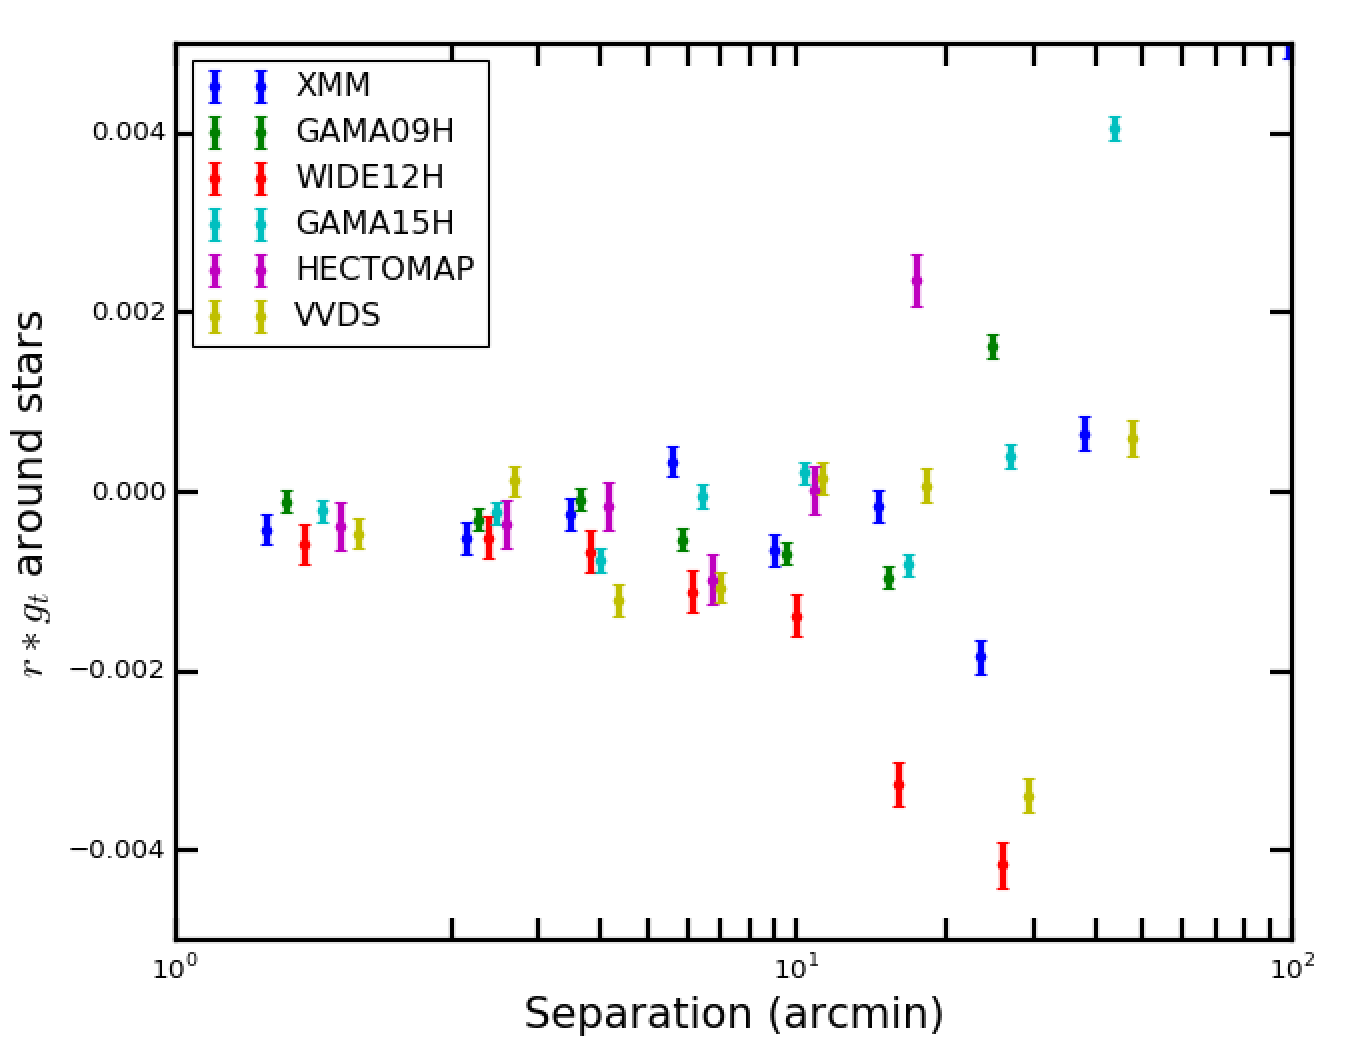
\includegraphics[width=0.4\textwidth]{gt_star.png}
    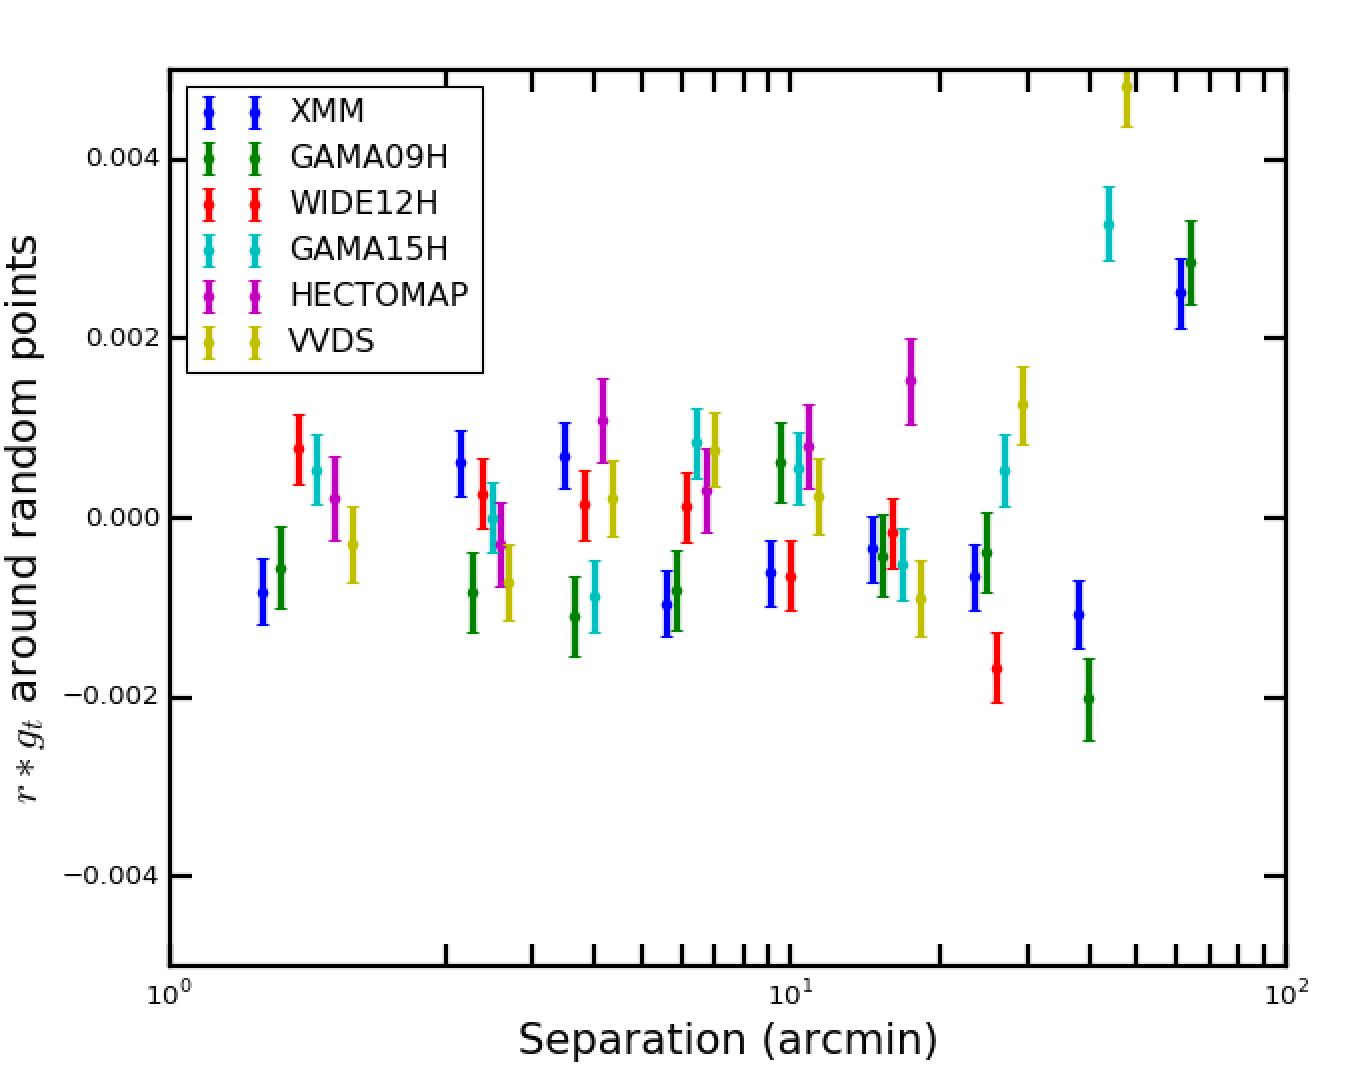
\includegraphics[width=0.4\textwidth]{gt_random.png}
    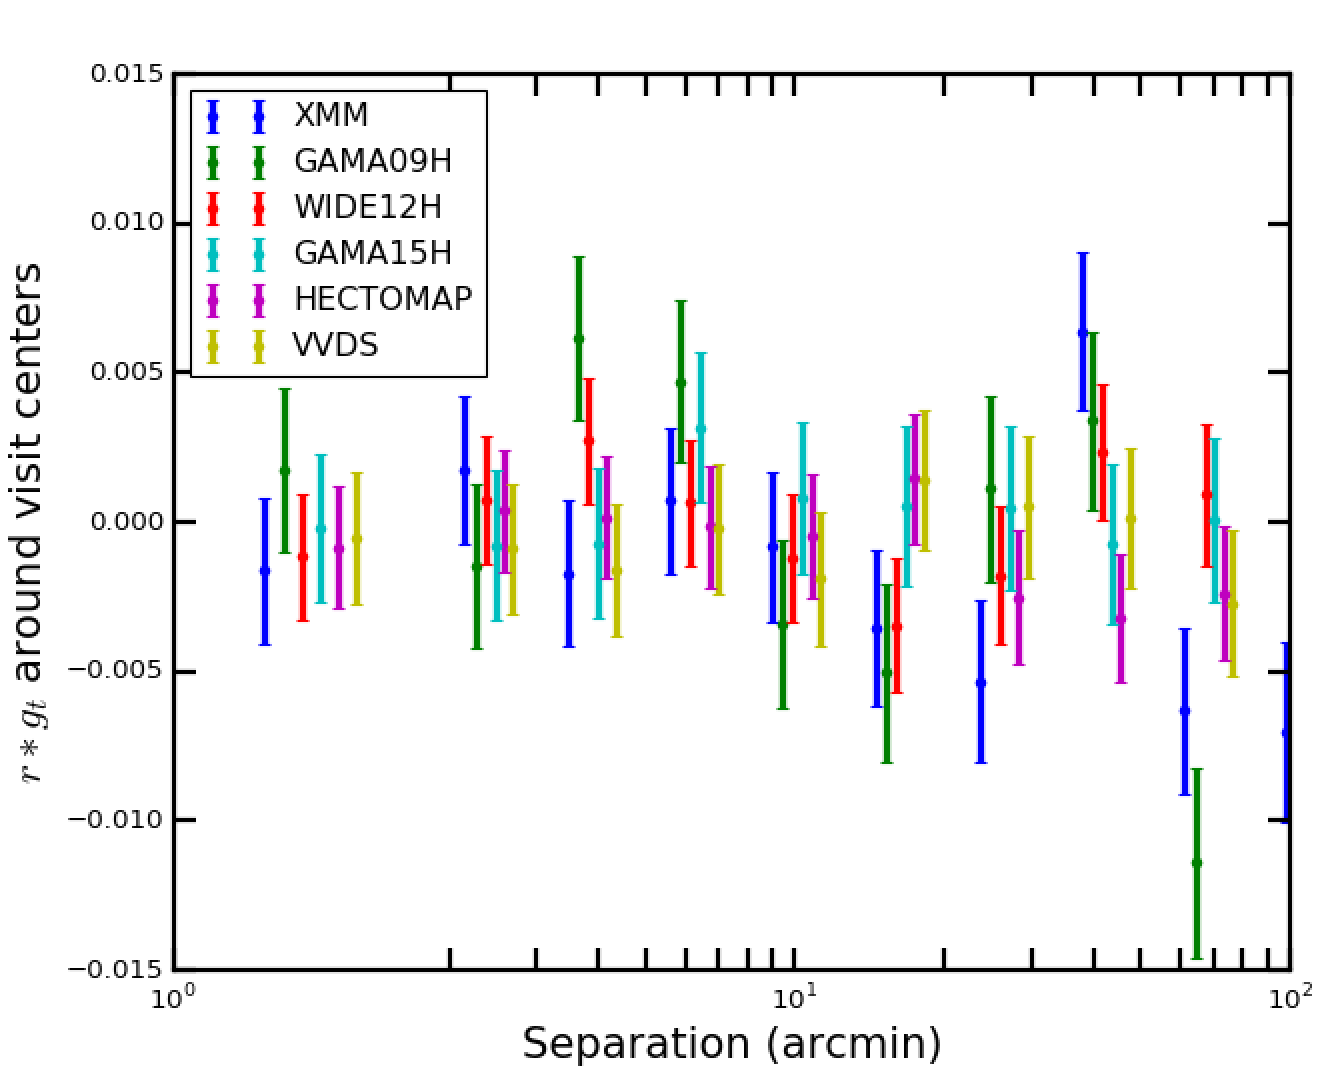
\includegraphics[width=0.4\textwidth]{gt_visit.png}
    \caption{
    The measured tangential shear by BFD around stars (top right), random points (top left) and $i$-band visit centers (bottom).  We measure this for each field separately.  Errors do not include cosmic variance, only shape noise.
    }
    \label{fig:gt_null}
\end{figure*}

\subsection{B-modes}

Lensing produces a purely "E-mode" convergence signal.  Examining the "B-mode" of the convergence can be a test for uncorrected systematic errors.  We measure the convergence by binning the $PQR$ values into square pixels of size 4\arcmin$\times$4\arcmin and calculating $g_1$ and $g_2$ for each bin.  We mask pixels where the number of galaxies is $\leq 250$ by setting $g_1$ and $g_2=0$ to avoid problems with too few galaxies (see Section ~\ref{Sec:Number}).  Convergence maps are then computed using the method in ~\cite{1993ApJ...404..441K}. We measure the errors on the convergence by randomly rotating the $PQR$ values 100 times and re-deriving the convergence maps for each realization.  The convergence maps are also then smoothed with a Gaussian filter of size 5\arcmin.  Figure \ref{fig:bmode} shows a histogram of the "E-mode" and "B-mode" convergence $S/N$ values for all unmasked pixels in the survey.  We fit the "B-mode" data to a Gaussian and see that it agrees, for the most part, with expectations.  There is some evidence of PSF leakage in the "B-mode" that was seen in \cite{ShearPaper:inprep}, which may account for the deviations seen.

\begin{figure}
    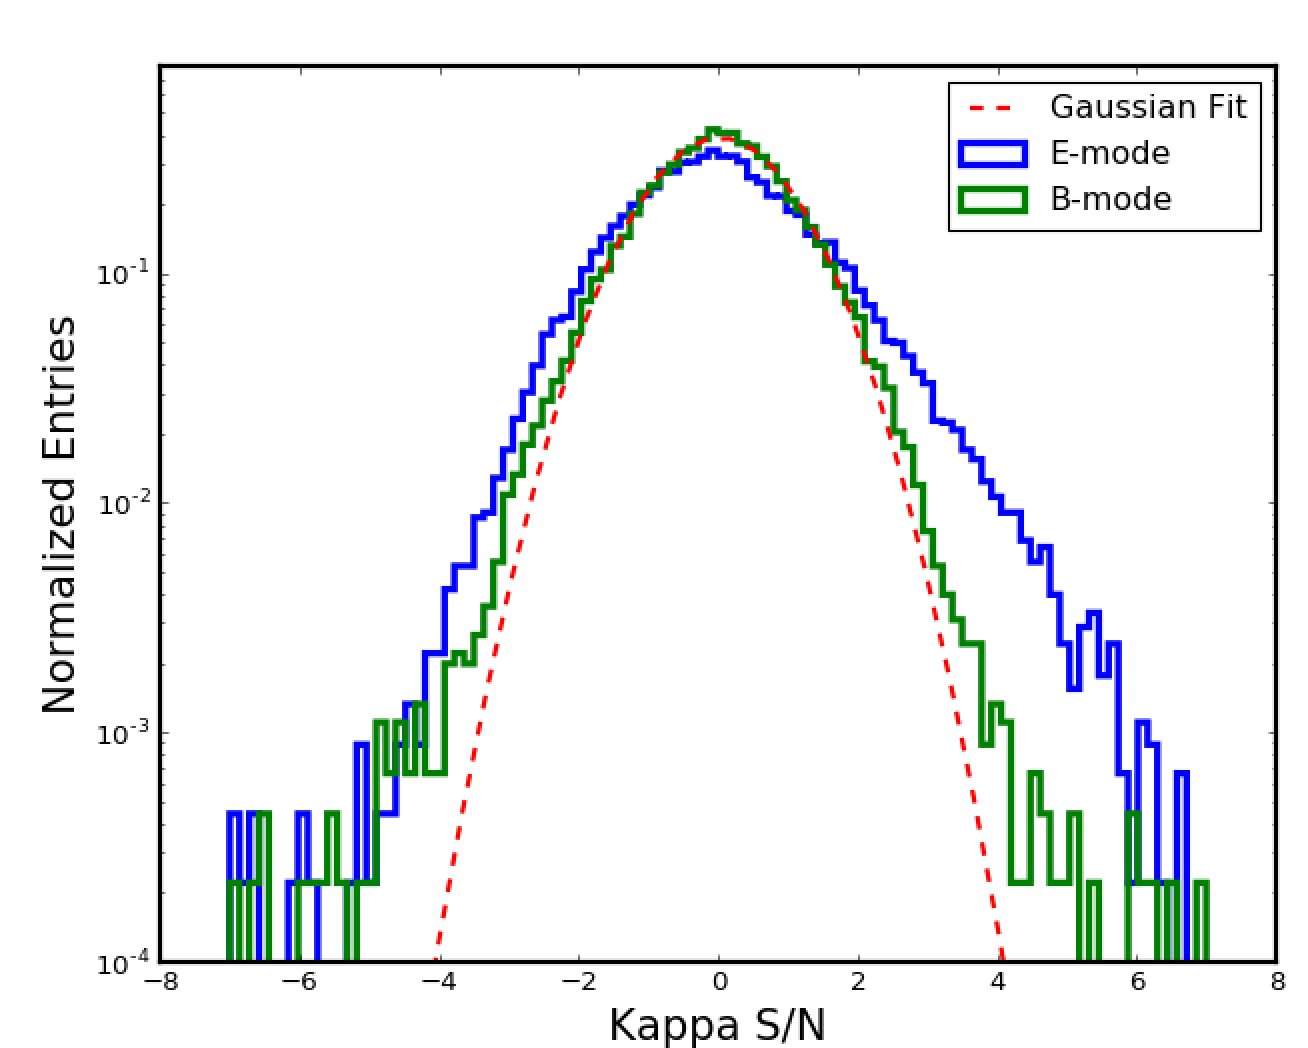
\includegraphics[width=0.5\textwidth]{bmode.png}
    \caption{
    A plot of the kappa "E-mode" (blue) and "B-mode" (green) $S/N$ values as measured from a combination of all the HSC fields.  The red line is a Gaussian fit to the "B-mode".
    }
    \label{fig:bmode}
\end{figure}


\subsection{PSF anisotropy leakage}
For each source, we can model the shear as being composed of the true shear plus additional systematics:
\begin{equation}
\vecg_{\rm m} = \vecg_{\rm true} + \alpha \vece_{\rm PSF} + c
\end{equation}
where $\vecg_{\rm m}$ is the measured shear, $e_{\rm PSF}$ is the PSF ellipticity and $c$ an additive term.  If we have not fully removed the PSF from the measurement we can measure a non-zero value of alpha.  We compute mean of the posterior of $\alpha$, $P(\vecg,\alpha|Data)$ by modifying slightly the BFD formalism.
dSpecifically, for each field we solve for the average shear over the field \vecg$_{\rm field}$ and $\alpha$:
\begin{equation}
\vecg_{\rm m} = \vecg_{\rm field} + \alpha(\vece_{\rm PSF}-\langle\vece_{\rm PSF}\rangle),
\end{equation}

where $\langle\vece_{\rm PSF}\rangle$ is the average PSF ellipticity for each field. To avoid spurious correlations due to the fact the mean PSF ellipticity is non-zero, we need to subtract of the mean PSF ellipticity.  This can be solved using:

\begin{multline}
%P(\vecg_{\rm{field}},\alpha|\rm{Data}) \approx -\sum_i \vecg_{\rm m}\cdot\left (\frac{\vecQ_i}{P_i} - n\Omega Q_{\rm sel} \right) \\
P(\vecg_{\rm{field}},\alpha|\rm{Data}) \approx -\sum_i \vecg_{\rm m}\cdot \vecQ_{\rm tot}
+ \frac{1}{2}\sum_i  \vecg_{\rm m}\cdot \matR_{\rm tot}
%\left(\frac{\vecQ_i\vecQ_i^T}{P_i^2} - \frac{\matR_i}{P_i} + n\Omega R_{\rm sel} \right)
\cdot \vecg_{\rm m},
\end{multline}
plugging in the value of $\vecg_{\rm m}$, and using linear algebra to solve for $g_{\rm field}$ and $\alpha$.

For the star sample we use the measured ellipticities of PSF stars on the coadd.  We compute separate values of $\alpha$, $\vecg_{\rm {field}}$ for all pairs of stars and galaxies at a given separation.   Figure \ref{fig:alpha} shows a plot of the posterior of $\alpha$ as a function of separation.  If there is uncorrected PSF ellipticity in the galaxy data due to either problems in the modeling or shear estimation this will not be consistent with zero.  The measured PSF leakage is small or consistent with zero for all fields.  

\begin{figure}
    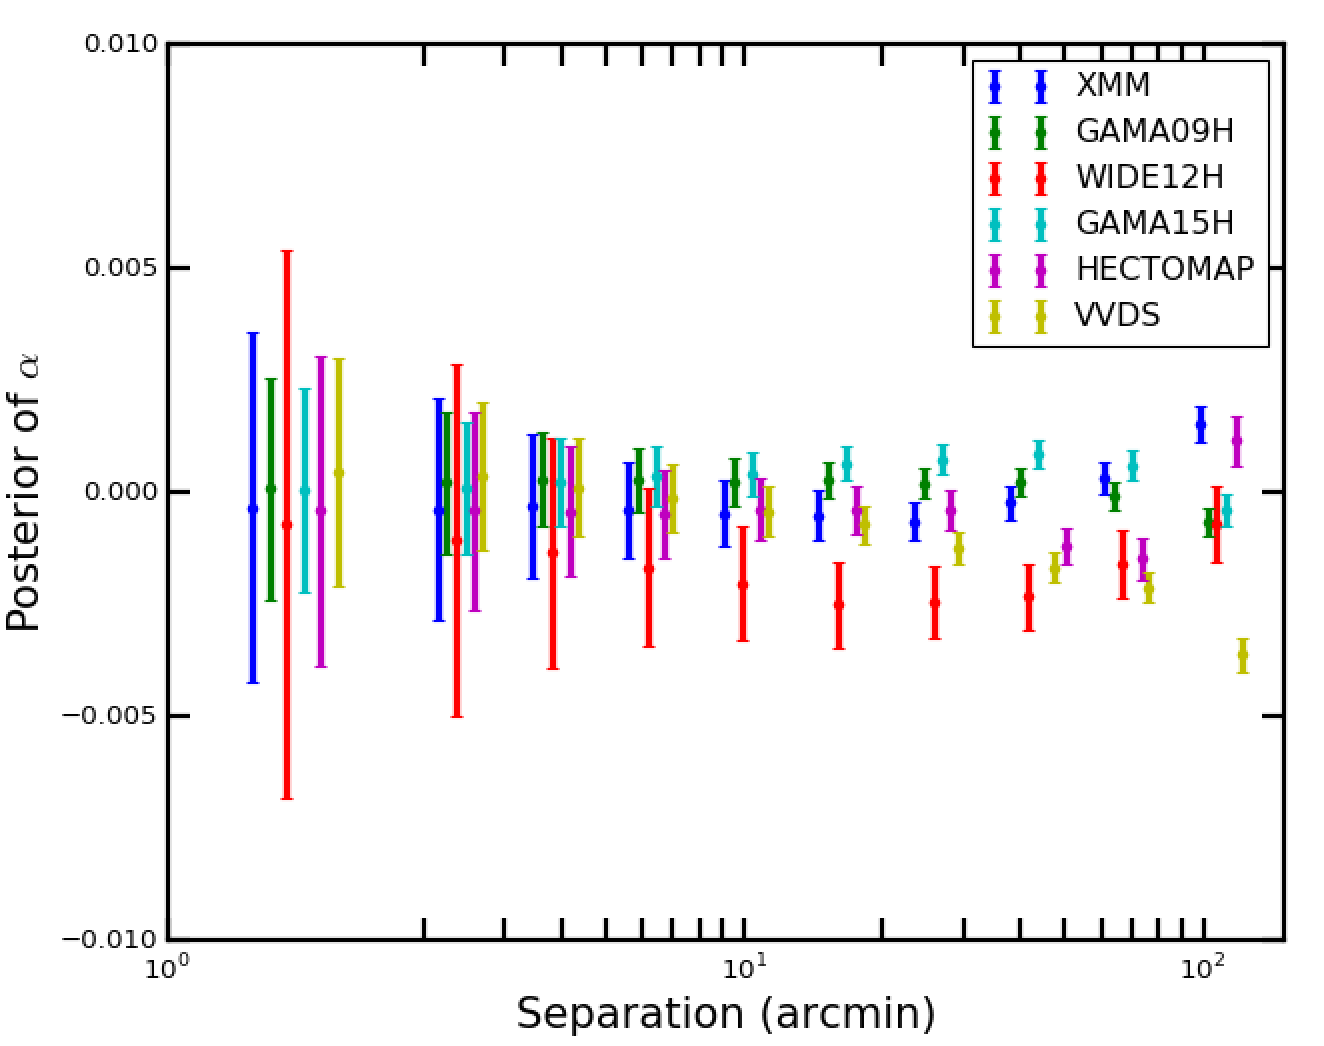
\includegraphics[width=0.5\textwidth]{alpha.png}
    \caption{
    The posterior of $\alpha$ (y-axis), a measure of the PSF anisotropy leakage, for different fields.  This is measured on all pairs of stars and galaxies within a given separation (x-axis).
    }
    \label{fig:alpha}
\end{figure}

\subsection{Consistency between samples}
\label{Sec:Data:Samples}

Typically, in weak lensing surveys the catalog is divided into different samples and compared to check for consistent results.  For BFD, we cannot arbitrarily make such cuts and have a valid prior.  However, we can make measurements on the low and high flux bins and for different noise bins because we have constructed separate priors for each of these samples.   We measure the stacked lensing profile, $\Delta\Sigma$, around a set of lenses.  This is defined as:

\begin{eqnarray}
\gamma_T & = & \frac{\Delta\Sigma} {\Sigma_{\rm cr}} \\ 
\Sigma_{\rm cr}(z_s,z_l) & = & \frac{c}{4\pi G} \frac{D_s}{D_l D_ls},
\end{eqnarray}
where $D_s,D_l$ and $D_ls$ refer to the angular diameter distance for the source, lens and between source and lens.

For each lens-source pair we compute the average $\langle\Sigma_{\rm cr}^{-1}\rangle$:
\begin{eqnarray}
\langle\Sigma_{\rm cr}^{-1}\rangle = \int_{z_l}^{\infty} \Sigma_{\rm cr}^{-1}(z_s,z_l)p(z_s)dz_s
\end{eqnarray}
where we have averaged over $p(z)$, the photo-z probability distribution.  Combining these together, we can compute the posterior of $\Delta\Sigma$ for a single lens by using:
\begin{eqnarray}
\vecQ_{\Delta\Sigma} & = & -\sum_i \frac{\vecQ_i \langle \Sigma_{\rm cr}^{-1}\rangle_i}{P_i} + \widetilde{\langle\Sigma_{\rm cr}^{-1}\rangle} n\Omega \vecQ_{\rm sel} \\
\matR_{\Delta\Sigma} & = &  \sum_i \langle\Sigma_{\rm cr}^{-1}\rangle_i^2 
\left(\frac{\vecQ_i\vecQ_i^T}{P_i^2} - \frac{\matR_i}{P_i}\right)\\
&  & + \widetilde{\langle\Sigma_{\rm cr}^{-1}\rangle}^2 n\Omega \matR_{\rm sel} \nonumber,
\end{eqnarray}
where $\widetilde{\langle\Sigma_{\rm cr}^{-1}\rangle}$ is the average $\langle\Sigma_{\rm cr}^{-1}\rangle$ over all of the objects within the specified radius around the lens.  (Need to double check that this is the correct way to handle the selection terms).  We can compute, as before, $\Delta\Sigma=\matR_{\Delta\Sigma}^{-1}\vecQ_{\Delta\Sigma} $.

Figure \ref{fig:dsigma_consistent} shows a comparison of the $\Delta\Sigma$ profile around red-sequence galaxy clusters as found by the CAMIRA \citep{Camira:inprep} cluster finder.  We split the clusters into a high and low redshift bin to test for differences as a function of redshift.  We can see that these seem to be in agreement within the error bars. (I need to figure out what is happening at large separations for the low/high noise comparison)


\begin{figure*}
    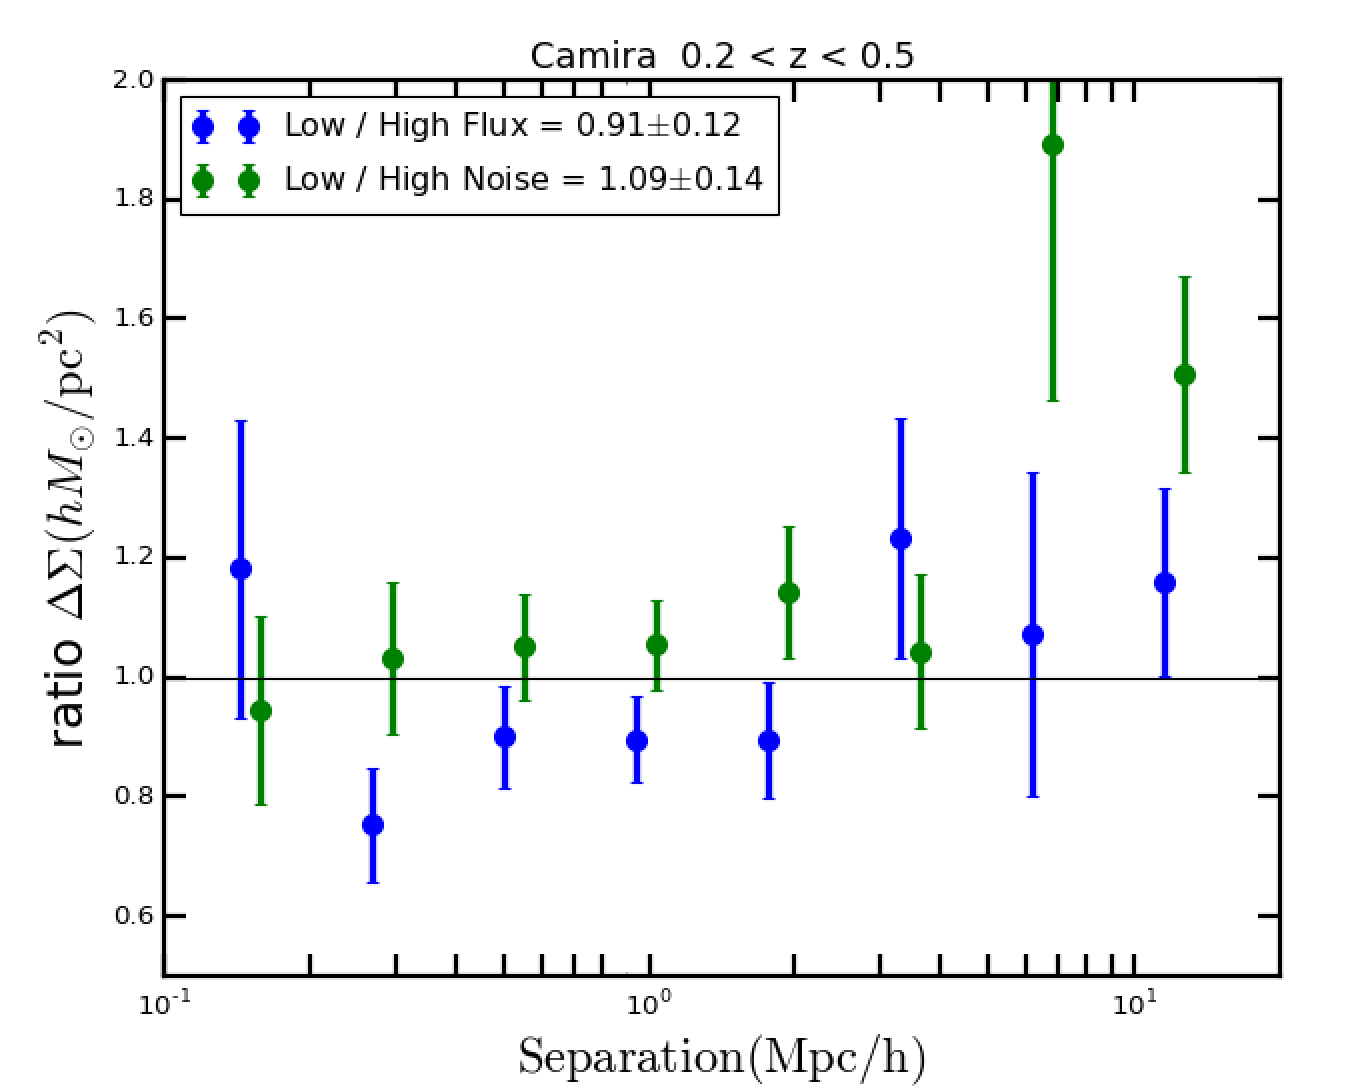
\includegraphics[width=0.45\textwidth]{dsigma_consistent_lowz.png}
    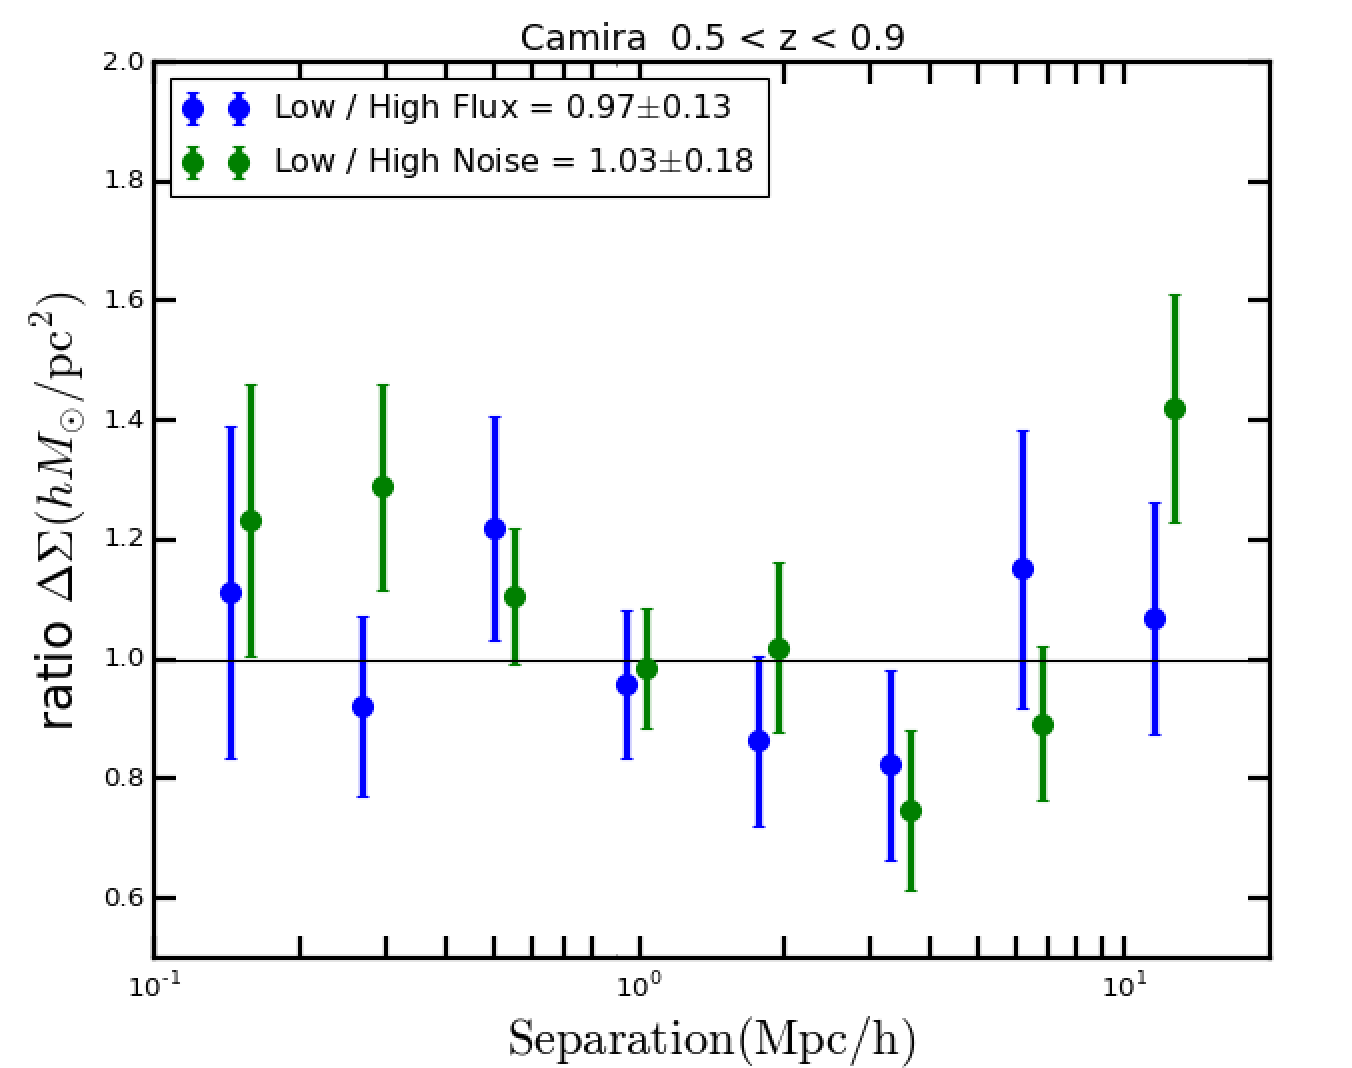
\includegraphics[width=0.45\textwidth]{dsigma_consistent_highz.png}
    \caption{
    $\Delta\Sigma$ profiles around CAMIRA clusters, low redshift (righg), high redshift (left) for different subsamples of objects.
}
    \label{fig:dsigma_consistent}
\end{figure*}



\section{Comparison with re-Gaussianization}
\label{Sec:Comparison}

A critical validation is that the shear signal from the re-Gaussianization method described in \cite{ShearPaper:inprep} is consistent with BFD.  Given the very different approaches of these methods, showing agreement gives confidence in the resulting shear catalogs. The number of objects selected by the two methods is roughly the same, however only 60$\%$ of the objects are in common.  Figure \ref{fig:bfd_hsm_flux_sn} shows the flux $S/N$ for objects selected from the two different methods as compared with the full catalog.  We can see that the biggest difference between the two is that re-Gaussianization selects more high $S/N$ objects due to no explicit maximum $S/N$ cut.  BFD selects more objects in the overlap region due to the single flux cut, compensating for the missing objects at higher $S/N$.

\begin{figure}
    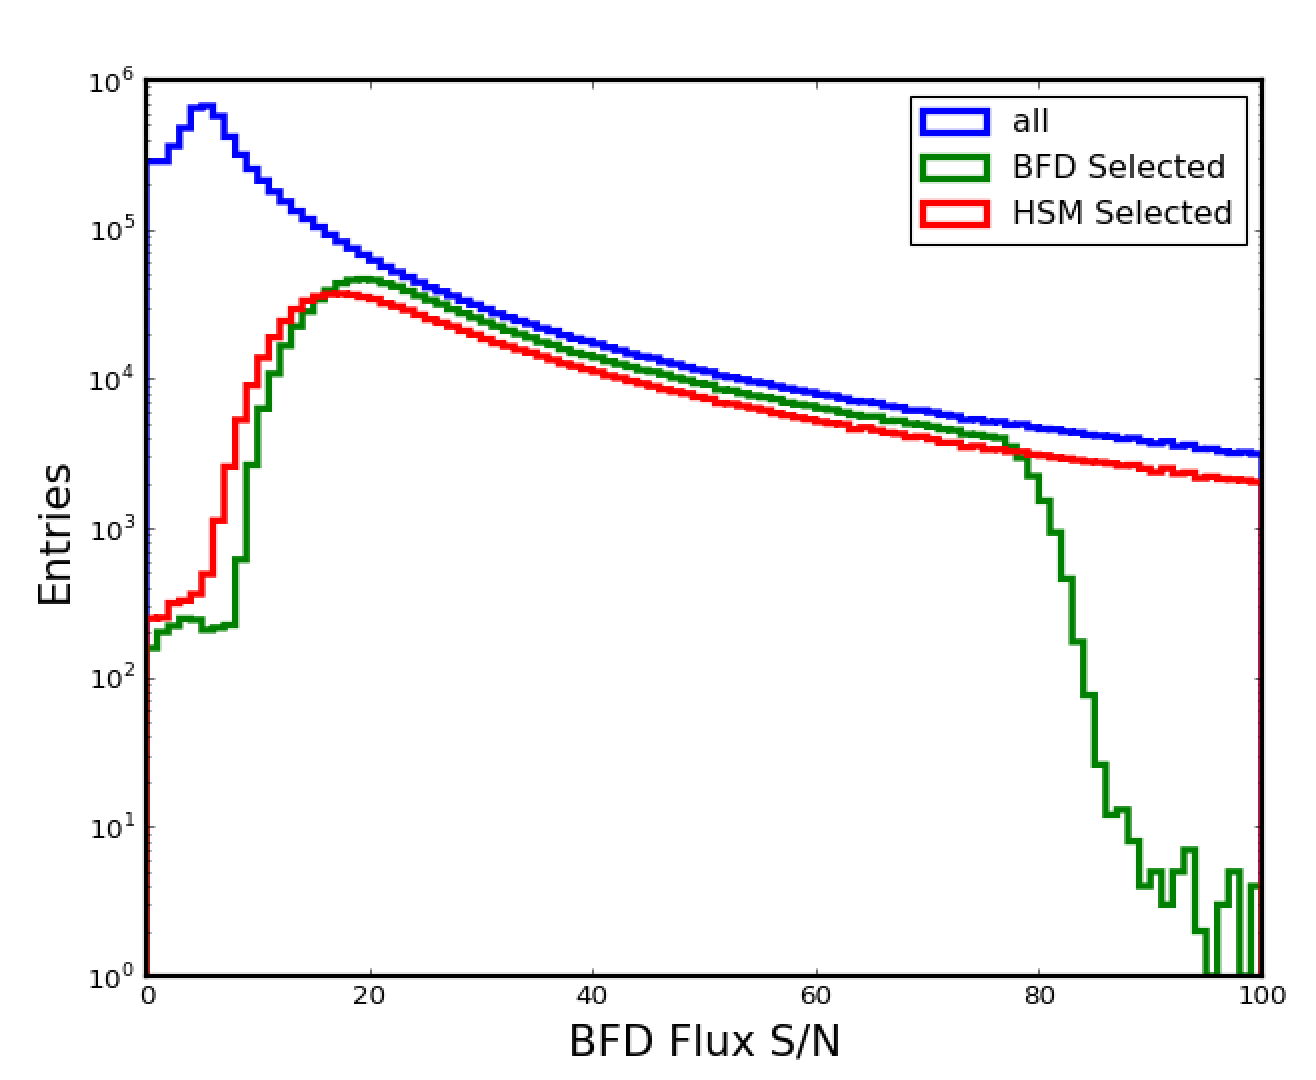
\includegraphics[width=0.5\textwidth]{bfd_hsm_flux_sn.png}
    \caption{
    A comparison of the S/N for objects for all objects (blue) and those selected by the BFD (green) and HSM (red).}
    \label{fig:bfd_hsm_flux_sn}
\end{figure}

In Figure \ref{fig:dsigma_hsm}, we compare the $\Delta\Sigma$ profiles around the same \texttt{CAMIRA} clusters as in \ref{Sec:Data:Samples}.  This shows excellent agreement between the two methods with no statistically significant bias.


\begin{figure*}
    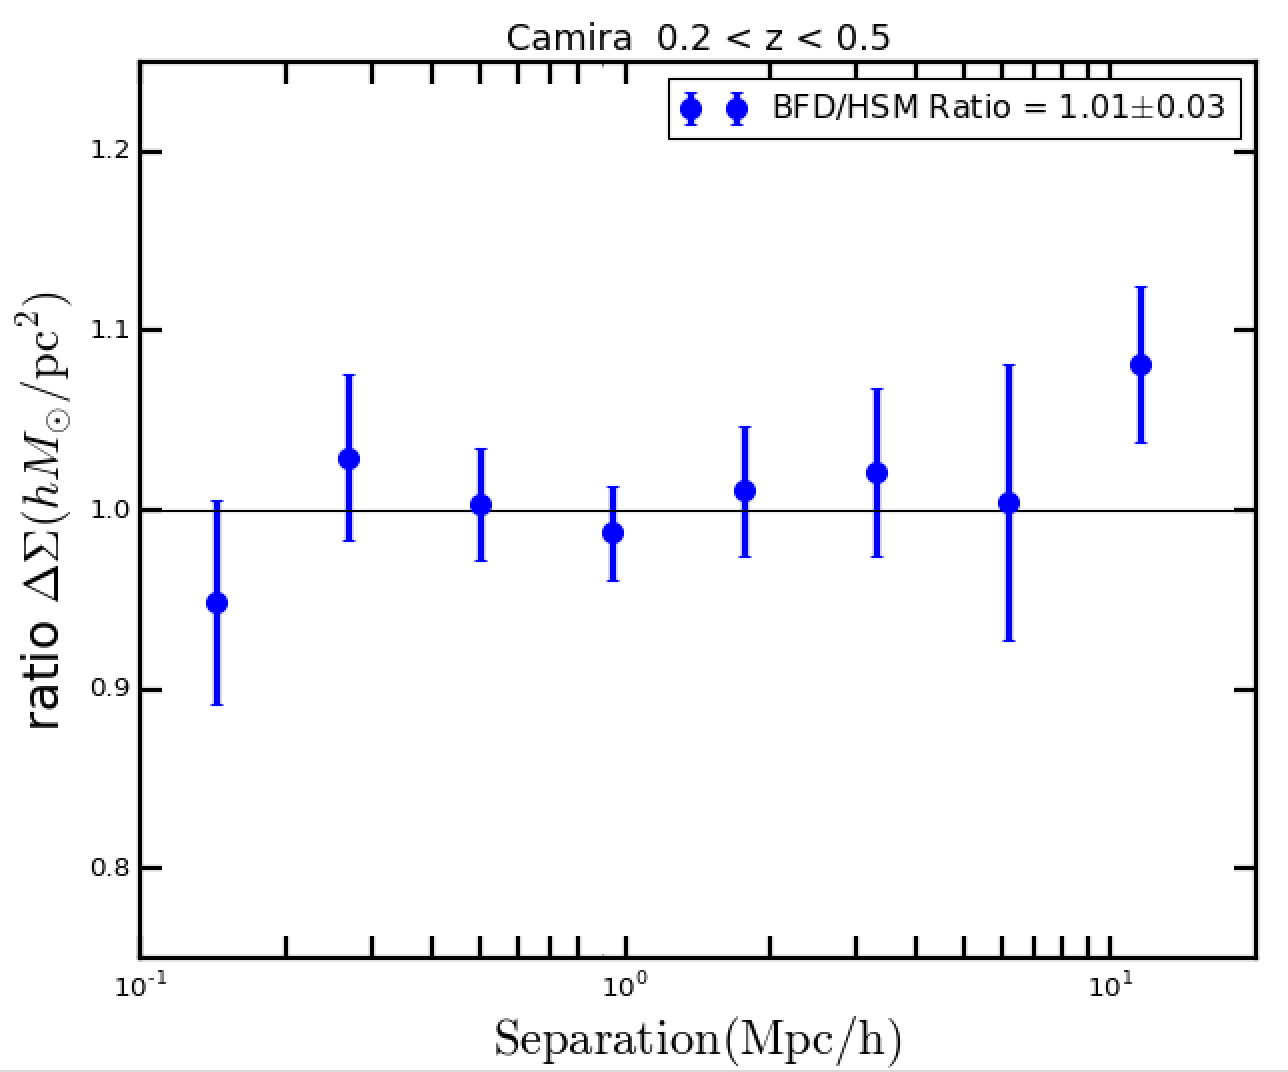
\includegraphics[width=0.45\textwidth]{bfd_hsm_lowz.png}
    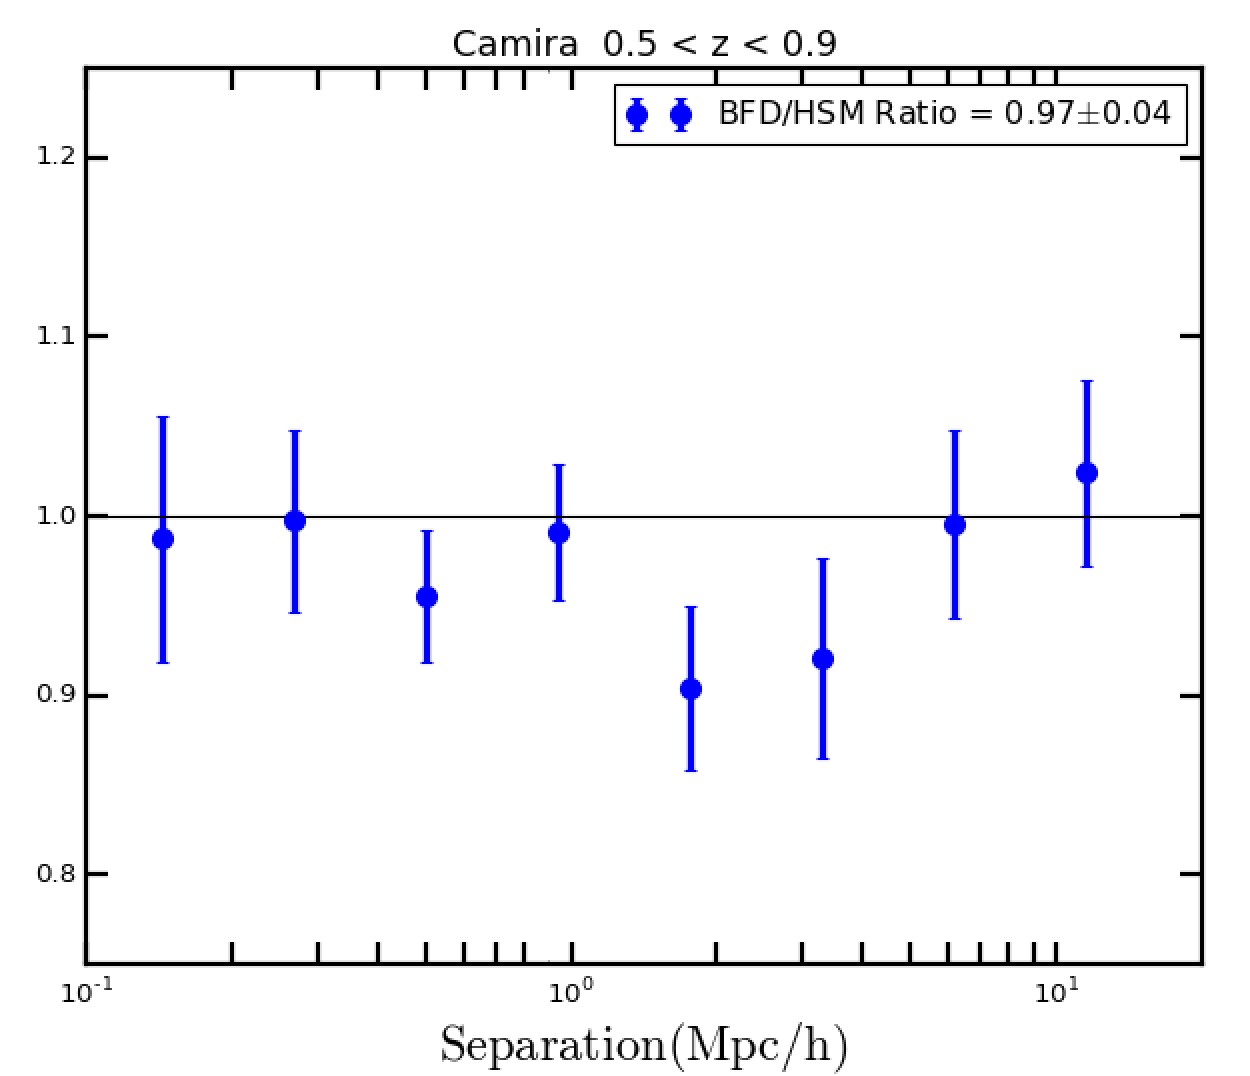
\includegraphics[width=0.44\textwidth]{bfd_hsm_highz.png}
    \caption{
    The ratio (BFD/HSM) of the $\Delta\Sigma$ profiles around \texttt{CAMIRA} clusters. Low redshift clusters are shown on the right and high redshift clusters on the left.
    }
    \label{fig:dsigma_hsm}
\end{figure*}

\section{Using the catalog}
\label{Sec:Catalog}
\subsection{Final Selection}

Here is a list of the final set of selection cuts:
\begin{enumerate}
\item Object be in FDFC region and outside of bright star mask
\item $0.1 \leq$ Flux variance $\le 1.2$
\item BFD magnitude $\le 24.6$
\item Flux $S/N \le 80$
\item $P \ge 0.01$

\end{enumerate}



\subsection{Known Issues}
\subsubsection{Outliers}
A small fraction of galaxies have small values of $P$.  This means they had few prior objects near them in moment space.  When included, these galaxies bias the shear estimate because they get a large weight from the ratio term $\vecQ_i/P_i$.  Figure \ref{fig:p_outliers} shows the number of objects as a function of $P$ for both data and simulations.  It can be seen that there is a higher population of low $P$ objects in the data compared to the simulations.  After examining these galaxies, many of them seem to be either artifacts, noise or detections in the outskirts of bright, nearby galaxies.  Figure \ref{fig:outliers} shows a random selection of some of these low $P$ galaxies.  To remove these, we place a cut at $P>0.01$.  We confirmed that changing this cut using values down to 0.005 had little impact on the resulting stacked lensing signals.


\begin{figure}
    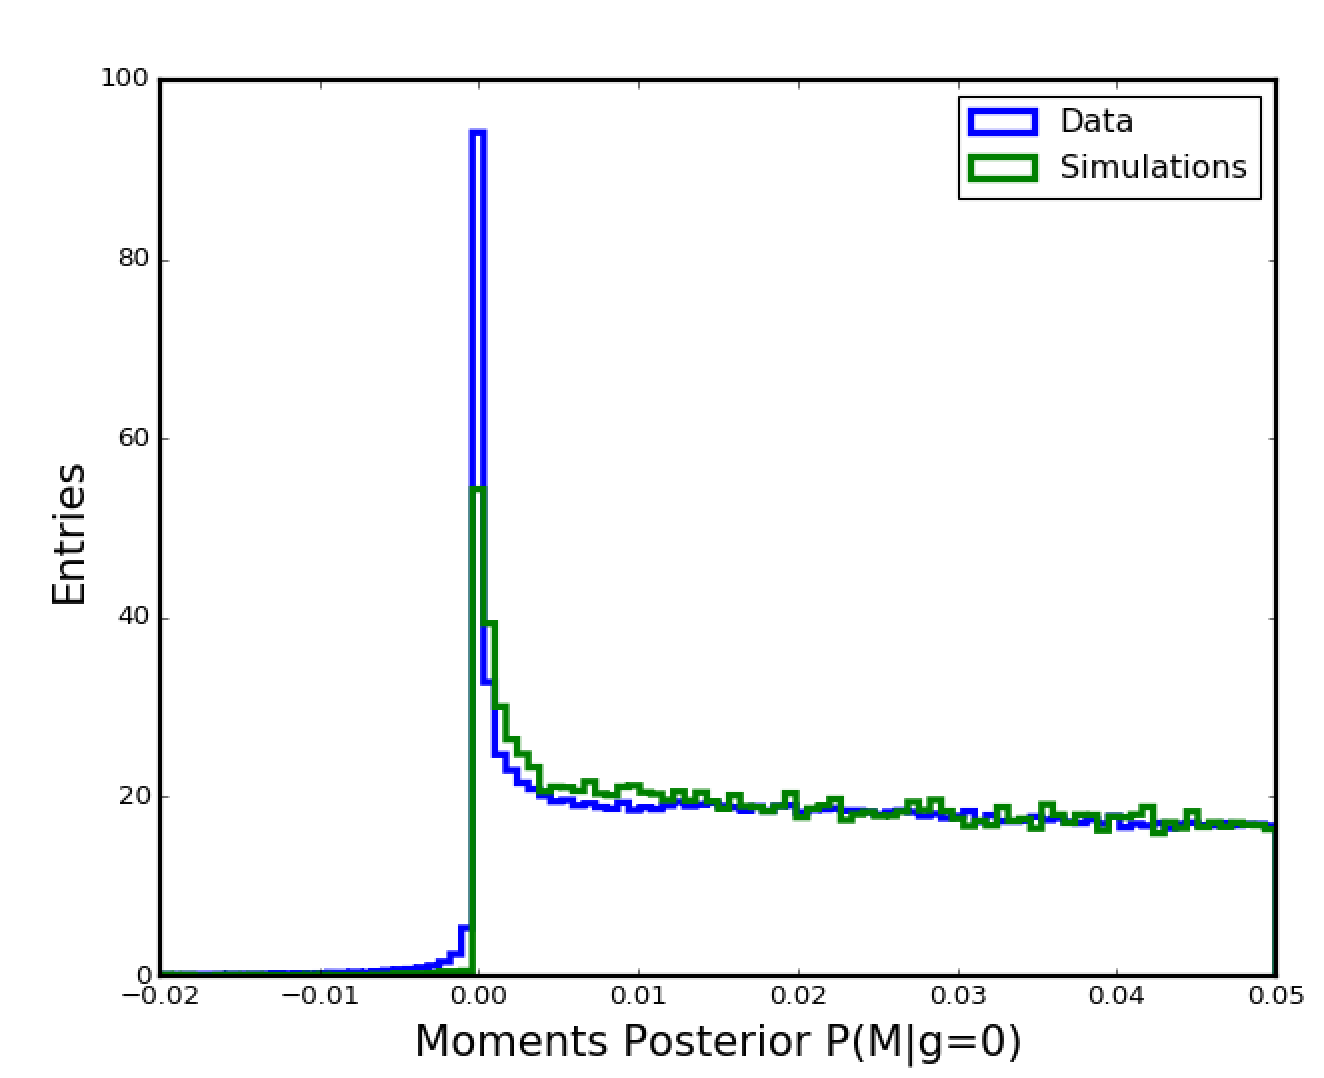
\includegraphics[width=0.5\textwidth]{outliers.png}
    \caption{
    The distribution of $P$ values for data (blue) and simulations (green).
    }
    \label{fig:p_outliers}
\end{figure}


\subsubsection{Number of galaxies}
\label{Sec:Number}
When calculating the shear from \vecQ and \matR, if there are not enough galaxies in the sample we fail the assumption that the posterior is Gaussian.  The estimated shear can then become noisy and biased.  To avoid this we need to average over a sufficient number of galaxies so as to make the posterior Gaussian.  In practice we found that averaging over $\sim200-300$ objects was enough to satisfy this assumption.  This restriction will limit the range of scales that we can use in scientific analyses.  

\subsubsection{Correlation functions}

Since BFD is not a point estimator, single galaxy shear estimates cannot be used naively to compute shear-shear correlation functions.  As in the previous section, once the shear values are averaged over a large enough number of galaxies this should not be a problem.  We leave the development of better shear-shear estimators for BFD to future work.

\section{Summary}
\label{Sec:Summary}

In this paper we have presented the application of the BFD method to the first year HSC dataset.  We have shown on simulations and data that we meet the requirements set in ~\citep{ShearPaper:inprep} for first year weak lensing analyses.  Our results agree to high precision with the re-Gaussianized method as demonstrated by comparing the lensing signal on high and low redshift red-sequence selected galaxy clusters.

In the future we plan to add the following improvements to our method:
\begin{enumerate}
\item Incorporate galaxy colors into the BFD analyses to enable joint lensing+photo-z analyses and remove selection biases associated between the two methods.
\item Combine data from multiple filters
\item Run on individual visits instead of the coadd.  This requires planned improvements in the deblender to properly deblend the visit images using the coadded images.
\item Work in sky coordinates, properly taking into account the full WCS solution.
\item Improve the implementation to reduce the number of separate priors that need to be created.
\item Relax the Gaussian assumption of the posterior to enable probing at smaller scales.
\item Incorporate magnification
\end{enumerate}


\bibliographystyle{astroads}
\bibliography{references}

\newpage
\appendix

\section{Examples of low $P$ galaxies}
Figure \ref{fig:outliers} shows an example of low $P$ galaxies that we cut out of our analysis.  While some of these seem to be reasonable galaxies, many of these seem to be associated with junk detections in the outskirts of bright objects or artifacts that have not been removed from the catalog.
\begin{figure*}
    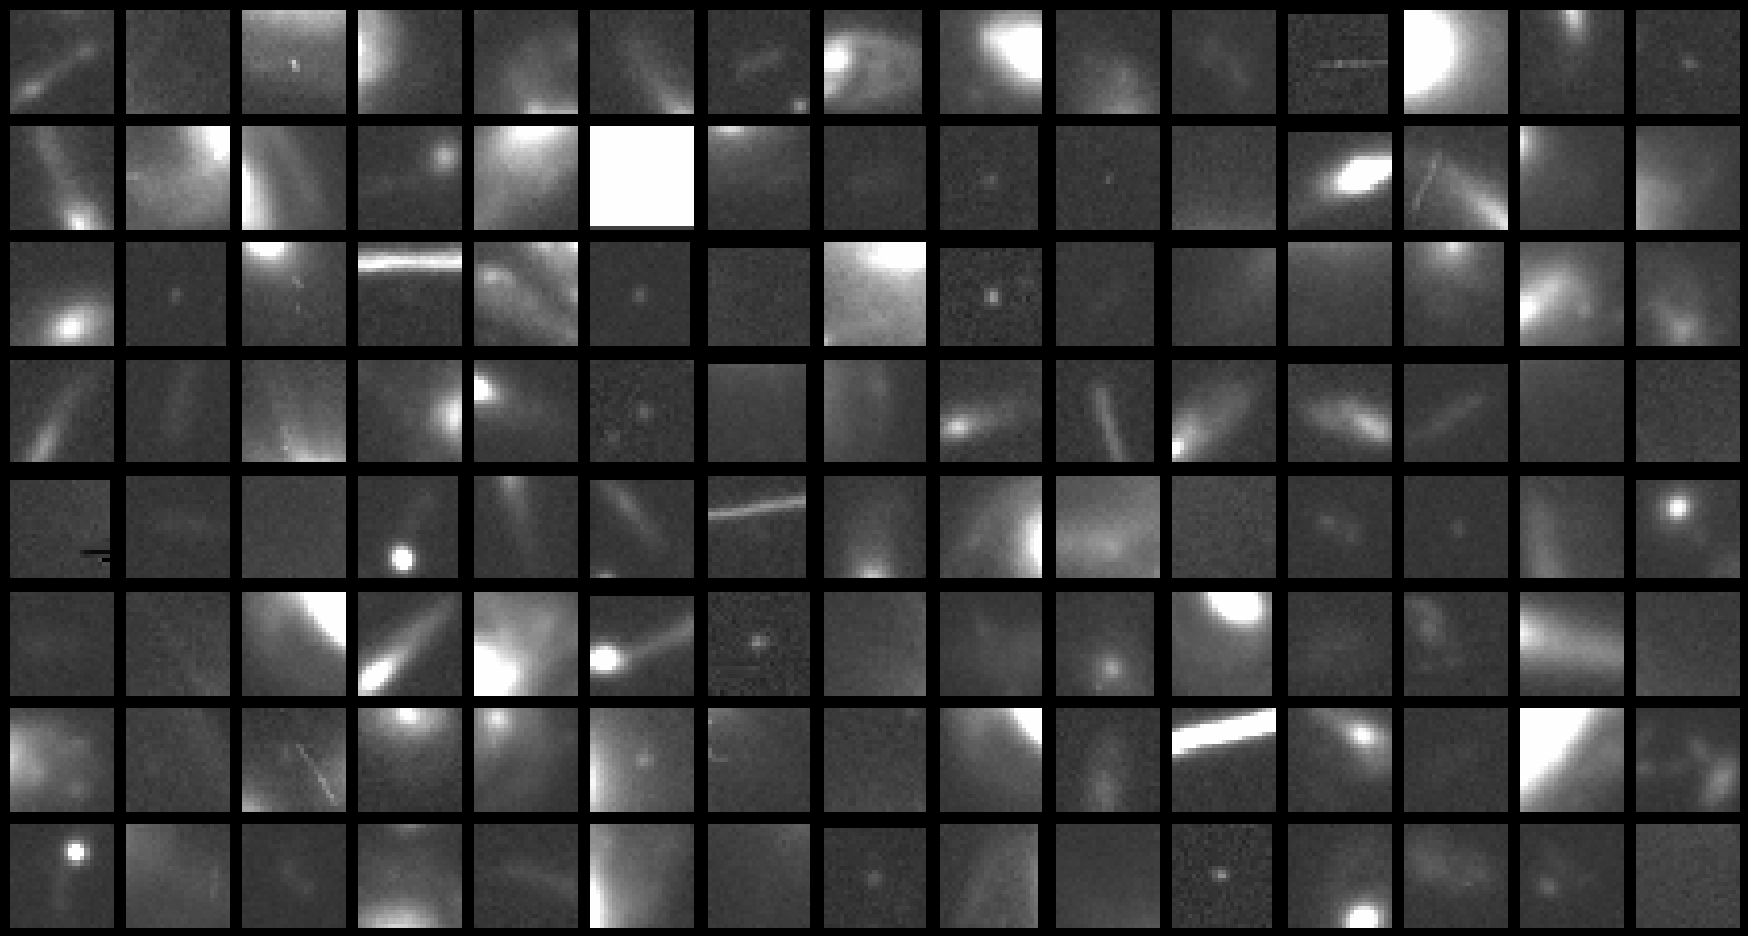
\includegraphics[width=\textwidth]{bad_examples.png}
    \caption{
    Postage stamps of galaxies with $P$ $< 0.01$.  The images are centered on the detected object.
    }
    \label{fig:outliers}
\end{figure*}





\section{Full Prior Distributions}
Figure \ref{fig:full_prior} shows the full set of moments and derivatives that are measured and used from the prior.  The first row are the raw moment distributions.
\begin{figure*}
    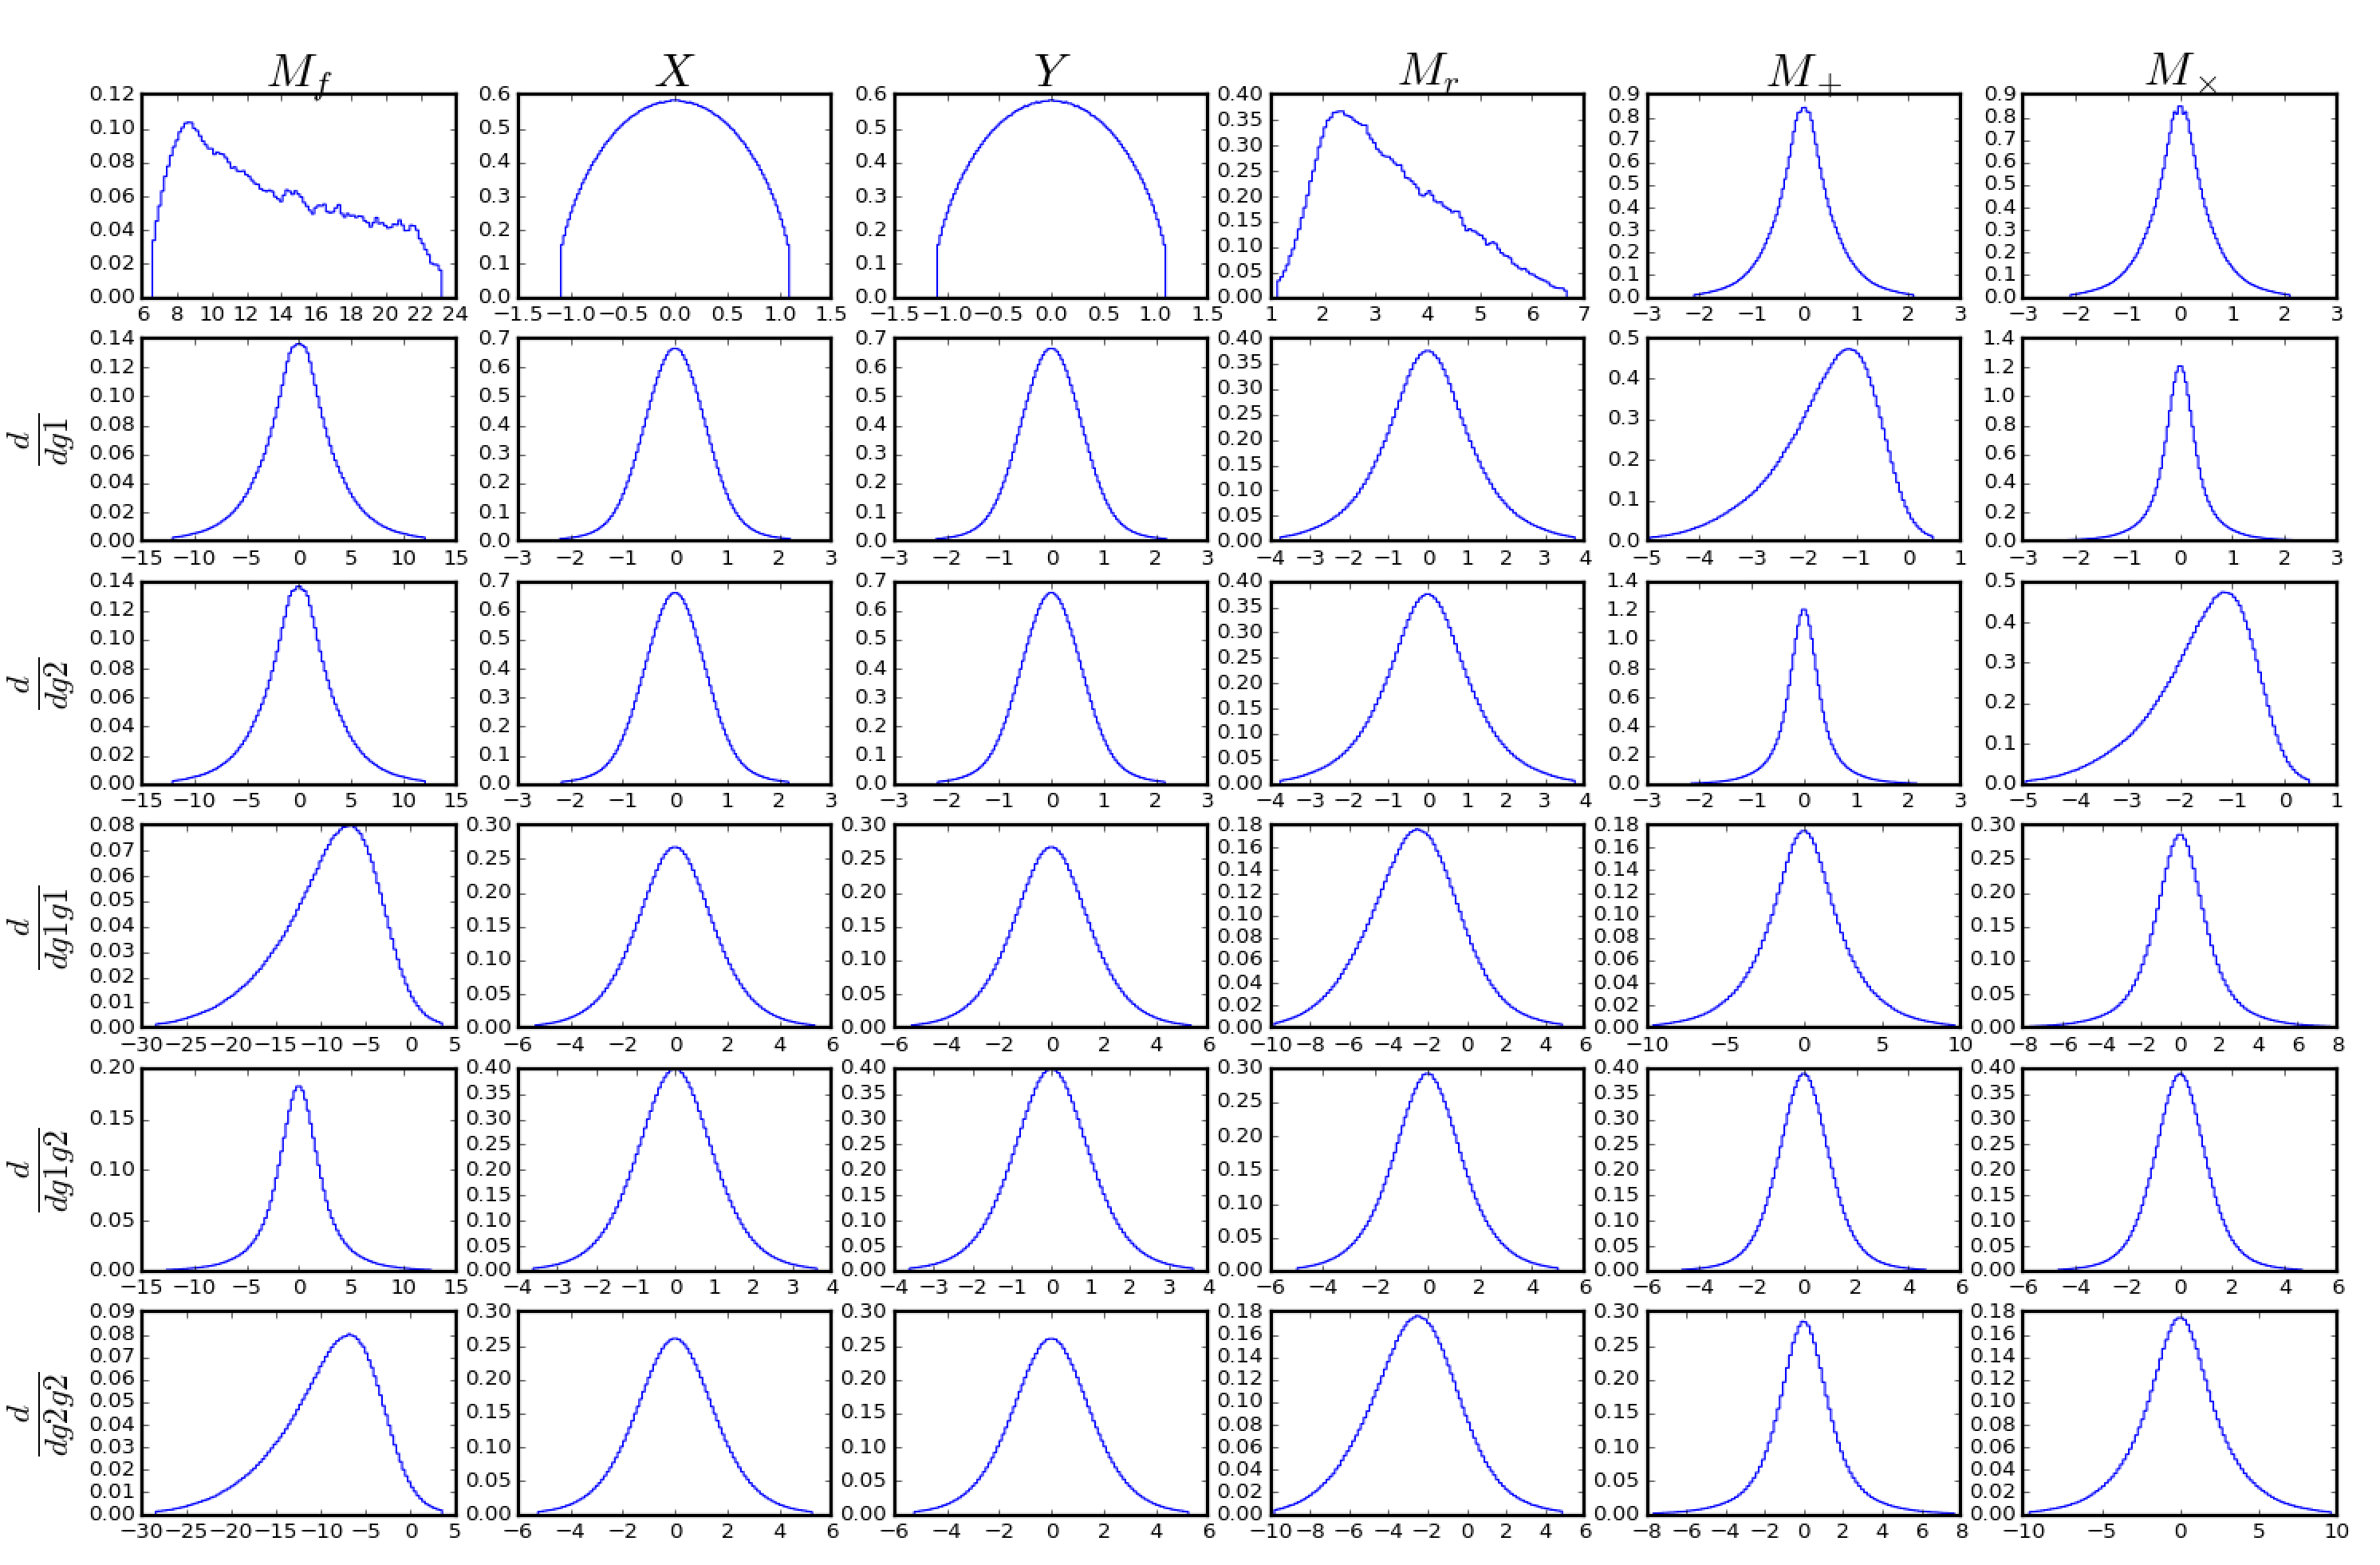
\includegraphics[width=\textwidth]{full_prior.png}
    \caption{
       Full set of prior distributions used in calculating the $PQR$ values.  The columns are different moments and the rows are derivatives with respect to shear.
    }
    \label{fig:full_prior}
\end{figure*}

\end{document}


